%\documentclass[lineno]{jfm}
\documentclass[lineno]{JFM-FLM_Au}

\usepackage{graphicx}
\usepackage{mathtools}
%\usepackage{epstopdf,epsfig}
\usepackage{labelfig}
\usepackage[svgnames,x11names,table,dvipsnames]{xcolor}
%\usepackage{newtxtext}
%\usepackage{newtxmath}
%\usepackage{epsfig}
\usepackage{epstopdf}

\usepackage{natbib}
%\usepackage{hyperref}
%\hypersetup{
%    colorlinks = true,
%    linkcolor  = blue,
%    urlcolor   = blue,
%    citecolor  = blue,
%}
\usepackage[justification=justified]{caption}
\usepackage{subcaption}
\usepackage{amsmath,bm}
\usepackage{mathrsfs} 
\usepackage{rotating}

%%\usepackage[colorlinks=true,linkcolor=blue,citecolor=blue,urlcolor = blue]{hyperref}
\usepackage[nameinlink]{cleveref}
\crefname{equation}{equation}{equation}
\crefname{Equation}{Equation}{Equation}
\crefname{eqnarray}{}{}
\crefname{figure}{figure}{figures}
\Crefname{Figure}{Figure}{Figures}
\crefname{table}{table}{tables}

\usepackage{amsfonts}
\usepackage{booktabs}
\usepackage{lipsum}

%\usepackage{showframe}

\newtheorem{lemma}{Lemma}
\newtheorem{corollary}{Corollary}

% Commands for possessive citing and element citing (figure, section, table) 
\newcommand{\poscite}[1]{\citeauthor{#1}'s (\citeyear{#1})}
\newcommand{\elementcite}[2]{\citeauthor{#1} (\citeyear{#1}; #2)}

\newcommand{\RomanNumeralCaps}[1]

\lefttitle{F. Espinoza, V. Ortiz, N. Vriend and T. Trewhela}
\righttitle{Journal of Fluid Mechanics}

\title{Internally-segregated structure of bidisperse hydraulic dunes}

\author{Felipe Espinoza\aff{1}, Vicente Ortiz\aff{1}, Nathalie Vriend\aff{2} \and Tomás Trewhela\aff{1}}

\affiliation{\aff{1} Facultad de Ingenier\'ia y Ciencias, Universidad Adolfo Iba{\~n}ez, Vi{\~n}a del Mar, Chile.
\aff{2} Paul M. Rady Department of Mechanical Engineering,
University of Colorado, Boulder, CO, USA}

\corresau{Felipe Espinoza, \email{feliespinoza@alumnos.uai.cl}}

\begin{document}
\maketitle

\begin{abstract}
This file contains information for authors planning to submit a paper to the {\it Journal of Fluid Mechanics}. The document was generated in {\LaTeX} using the JFM class file and supporting files provided on the JFM website \href{https://www.cambridge.org/core/journals/journal-of-fluid-mechanics/information/author-instructions/preparing-your-materials}{here}, and the source files can be used as a template for submissions (please note that this is mandatory for {\it JFM Rapids}). Full author instructions can be found on the \href{https://www.cambridge.org/core/journals/journal-of-fluid-mechanics/information/author-instructions}{JFM website}. The present paragraph appears in the \verb}abstract} environment. All papers should feature a single-paragraph abstract of no more than 250 words which must not spill onto the second page of the manuscript.
\end{abstract}

\begin{keywords}
Authors should not enter keywords on the manuscript, as these must be chosen by the author during the online submission process and will then be added during the typesetting process (see \href{https://www.cambridge.org/core/journals/journal-of-fluid-mechanics/information/list-of-keywords}{Keyword PDF} for the full list).  Other classifications will be added at the same time.
\end{keywords}

%{\bf MSC Codes }  {\it(Optional)} Please enter your MSC Codes here

%\section{First-order heading}
%\label{sec:headings}

%The layout design for the {\em Journal of Fluid Mechanics} journal has been implemented as a LaTeX\ style file.%
%\footnote{To know more information about LaTeX and its packages, try https://ctan.org/?lang=en}%
%The FLM style file is based on the ARTICLE style as discussed in the LaTeX\ manual. Commands which differ from the standard LaTeX\ interface, or which are provided in addition to the standard interface, are explained in this guide. This guide is not a substitute for the LaTeX\ manual itself.

%--------------------------------------------------------------
\section{Introduction}
\label{Sec:introduction}

%Dune formation and the flat-bed instability
Sand dunes are dynamic, self-organizing topographic structures formed by the complex interplay between a fluid (such as wind or water) and a granular bed, and they are ubiquitous across desert ergs, river beds and coastal environments \citep{charru2013,vriend2026dynamics,arrospide2018,Lapotre2017}. The life of a dune typically begins with a flat-bed instability, this arises from a phase lag between the sediment-transport flux and the bed topography: linear stability analyses of the coupled flow, transport and topography system show that the sediment flux reaches its maximum slightly upstream of the topographic crest, so that sediment converges and accumulates there, amplifying the bedform while simultaneously advecting it downstream \citep{charru2013,vriend2026dynamics}. This destabilizing mechanism operates, with variations in the details of the flow, in both aeolian and hydraulic settings \citep{charru2013,Lapotre2017,raudkivi2006}, and constitutes the classical paradigm from which the subsequent nonlinear growth, coarsening and migration of dunes are understood \citep{vriend2026dynamics}.

Once initiated, the migration of a dune is sustained by the continuous erosion of sediment from its upstream face (stoss) and its subsequent deposition on the downstream face (lee) \citep{kleinhans2004_34}. Three linked mechanisms drive this cycle. (i) The overlying fluid exerts a shear stress on the grains and, once this stress surpasses a critical threshold, particles are entrained by the flow \citep{gao2016}; grains then move up the windward slope mainly as bedload, by sliding, rolling, or bouncing (saltating) along the surface. (ii) As the fluid reaches the crest and passes the ``brink point'' of the dune, the flow separates from the surface, creating a turbulent recirculation zone, or wake, in the lee of the dune; in this low velocity zone grains lose momentum and settle out of the fluid like rain, a process known as grain fall \citep{anderson1988}. (iii) As grain fall accumulates sediment on the upper part of the lee slope, the slope eventually exceeds the sediment's angle of repose (typically around $30°$ for sand and similars) once this critical angle is surpassed, the mass of sand fails and moves down the slope as a high-concentration grain flow, or avalanche. This continuous cycle of avalanching pushes the dune forward and leaves behind the characteristic internal layered structure known as cross-stratification, or cross-bedding \citep{reesink2007,reesink2009,bristow2000}.

%add text of the experiments
Flume experiments of bidisperse hydraulic dunes provide empirical observations of internal sorting, showing the qualitative development of coarse-grain accumulation and cross-stratified deposits under controlled flow conditions. However, laboratory experiments do not easily isolate individual kinematic velocity fields, measure internal pressure distributions, or systematically explore broad parameter spaces of active-layer dynamics. Continuum mathematical models complement these experimental observations by providing a quantitative framework for analyzing internal bedform stratigraphy.

%Segregation and the internal architecture of bidisperse dunes
In nature, however, grains are rarely uniform in size: beds are polydisperse, and this size variation introduces an additional process that reshapes the internal structure of bedforms, namely size segregation \citep{blondeaux2012}. Size segregation in dunes is dictated by the physics of moving granular materials. In this agitated state, a dual mechanism operates: on the one hand, kinetic sieving occurs, whereby smaller grains are more likely to fall through the gaps that open beneath them; on the other hand, squeeze expulsion takes place, whereby larger grains are levered toward the surface to preserve a uniform volume fraction in the flow \citep{gray2005,Gray2018,trewhela2021}.

In polydisperse beds, shearing during slip-face avalanches causes vertical size segregation \citep{gray2005,trewhela2021}. As large grains reach the flow surface, they travel over a smoother bed of fine particles and gain momentum to roll down to the dune toe in a process known as overpassing \citep{reesink2007,kleinhans2004_34}. Conversely, fine grains experience greater friction and deposit higher on the slope, creating a spatial separation that leaves a geological record of cross-stratification \citep{gao2016,bristow2000}. Closely linked to this differential deposition is armoring, where the accumulation of large particles builds a protective pavement. Because coarse grains require higher shear stress for mobilization \citep{shields1936anwendung}, this layer stabilizes the bed and restricts vertical sediment exchange. In subaqueous systems, continuous winnowing of fine sand causes the armor layer to sink, eventually forming a solid, static floor at the maximum depth of the dune troughs \citep{blom2003,blom2008}.

%Numerical modelling of segregation
To examine this internal structure through the framework of segregation theory, we develop an analytical description of the governing equations and solve it numerically. The equations governing transport and segregation in sedimentary beds are nonlinear and usually lack a closed-form analytical solution, and they further exhibit discontinuities such as concentration fronts and shock waves \citep{savagehutter1989,gray2005}. To capture sharp fronts without spurious oscillations, high-resolution spatial reconstructions (MUSCL \citep{vanLeer1979} and WENO \citep{Liu1994,JiangShu1996,Henrick2005}) are combined with Rusanov Riemann solvers \citep{rusanov1961} and Strong Stability Preserving (SSP) Runge--Kutta time integration \citep{GottliebShuTadmor2001}, subject to the CFL condition \citep{CourantFriedrichsLewy1928}.. These techniques, consolidated in the conservation-laws literature \citep{toro2009}, have been applied successfully to granular segregation by \citet{Christov2017} and to shallow granular flows by \citet{Tai2015}, as well as in well-balanced schemes for sediment transport \citep{Burger2011,chiavassa2016}.

%Aim and outline of the paper
The primary benefit of these models lies in their ability to resolve the multiscale interaction that neither laboratory experiments fully capture: they reproduce the formation and migration of segregation interfaces, conserve mass exactly, giving access to internal variables that are difficult to measure experimentally. Most importantly, when validated against experimental data, these schemes bridge the gap between macroscopic bedload-transport models and microscopic segregation mechanisms, delivering a coherent predictive framework for the morphodynamics of bidisperse beds \citep{Christov2017,Tai2015}. 
%Despite this progress, a model that couples the bulk flow field of a migrating hydraulic dune to a bidisperse segregation-advection equation, and thereby predicts the internally segregated structure of the bedform itself, is still lacking.

%The specific modelling strategy adopted here follows three choices motivated by the physical picture above. First, rather than solving the full granular rheology for the coupled fluid–grain system, we prescribe a kinematic bulk velocity field for the migrating dune, in the spirit of reduced segregation models that impose an underlying flow structure and solve the resulting segregation-advection problem on top of it \citep{pearse2026}. Second, the segregation velocity magnitude $f_{sl}$ and the diffusivity $D_{sl}$ are built as a direct extension of the experimental scaling law of \citet{trewhela2021}, retaining its shear rate, pressure and grain size ratio dependence while introducing a decoupled shear scale and a pressure floor appropriate to the free surface of a dune. Third, and consistent with the armoring mechanism described above, both fluxes are confined to a thin near-surface active layer that vanishes smoothly with depth: once grains are advected below this layer they are effectively frozen, so that the model reproduces, by construction, the same separation between a mobile surface layer and a static, armoured substrate observed in nature \citep{gao2016,blom2008}. In \S\ref{Sec:segregation} we formulate the bidisperse particle-size segregation problem for a hydraulic dune; \S\ref{Sec:mathematical} presents the governing mathematical scheme and its numerical solution; \S\ref{Sec:results} discusses the resulting parameters and internal structure; and \S\ref{Sec:conclusions} summarizes the main conclusions of this work.


\section{Bidisperse particle-size segregation}
\label{Sec:segregation}

\subsection{Governing equations}
\label{Subsec:si}

Consider a bidisperse granular bed composed of large and small particles (subscripts $l$ and $s$, respectively) that together occupy a volume fraction $\Phi_v \in [0,1]$ of the dune, excluding the void space. From this we define the volume fraction of each species per unit granular volume as

\begin{equation}
    \phi_l = \frac{\Phi_l}{\Phi_l + \Phi_s}, \quad \phi_s = \frac{\Phi_s}{\Phi_l + \Phi_s}
    \label{eq:concentrations}
\end{equation}

Inside the dune the total solid volume fraction $\Phi = \Phi_l + \Phi_s$ remains constant \citep{bacik2020}; by definition, the two concentrations therefore satisfy $\phi_l + \phi_s = 1$

Using these bulk concentrations, the general form of the bidisperse segregation equations for the small particles (see, e.g., \citet{Gray2018}) reads

\begin{equation}
    \frac{\partial \phi_s}{\partial t} + \nabla \cdot (\phi_s \boldsymbol{u}) + \nabla \cdot \left( f_{sl} \phi_s \phi_l \frac{\boldsymbol{g}}{|\boldsymbol{g}|} \right) = \nabla \cdot (\mathcal{D}_{sl} \nabla \phi_s)
    \label{eq:OGformlarge}
\end{equation}

Each particle species obeys its own conservation law \citep{GajjarGray2014}. When both species share similar intrinsic density, summing these two equations cancels the segregation-flux terms and yields a divergence-free bulk velocity field, $\nabla \cdot \mathbf{u} = 0$


\subsection{Model parameterization}
\label{sec:parameterization}
%transform the eq to my system
To simulate the internal dynamics of a dune, a longitudinal cross-section is taken, yielding a 2D system (with $x$, $z$ axes). Focusing the system on the concentration of small particles, the general form of the bidisperse segregation equation \eqref{eq:OGformlarge} can be rewritten for this system as
\begin{equation}
    \frac{\partial \phi_s}{\partial t} + \frac{\partial (u\phi_s)}{\partial x} + \frac{\partial (w\phi_s)}{\partial z} + \frac{\partial F_{\mathrm{seg}}}{\partial z} = \frac{\partial}{\partial z}\!\left(D_{\mathrm{sl}}\,\frac{\partial \phi_s}{\partial z}\right),
    \label{eq:systemform}
\end{equation}
\begin{equation}
    F_{seg} = f_{sl} \phi_l \phi_s \frac{g}{|g|}
\end{equation}
Here, the closure terms for the segregation velocity coefficient $f_{sl}$ and the intergranular diffusion coefficient $D_{sl}$ adapt the model of \citet{trewhela2021}. The constitutive functions governing the intergranular dynamics are
\begin{align}
    \bar d(\phi_s) &= (1-\phi_s)\,d_l + \phi_s\,d_s, \label{eq:dbar}\\
    F(R,\phi_s) &= (R-1) + E(1-\phi_s)(R-1)^2, \label{eq:FRphi}\\
    f_{sl} &= \frac{B\,\dot\gamma\,\bar d^{\,2}}{C\,\bar d + p(x,z)}\,F(R,\phi_s), \label{eq:fsl}\\
    D_{sl} &= A\,\dot\gamma\,\bar d^{\,2}. \label{eq:Dsl}
\end{align}
The effective lithostatic pressure in the granular medium is
\begin{equation}
    p(x,z) = \Phi\,(h(x)-z) + p_{\mathrm{floor}}, \quad p_{\mathrm{floor}} = 3\,\Phi\,\delta_a,
    \label{eq:pressure}
\end{equation}
where $\Phi = 0.6$ is the solid packing fraction and $\dot\gamma$ is the shear rate (detailed in \S\ref{sec:shearrate}). At the free interface ($z \approx h(x)$), the granular hydrostatic pressure tends to zero, inducing a mathematical singularity in the segregation coefficient $f_{sl}$ [eq.~\eqref{eq:fsl}] that forced an overly restrictive numerical time step. Introducing the pressure floor $p_{\mathrm{floor}}$ models the minimum tensile resistance of the surface flow, so that segregation saturates rather than diverges; this regularization analytically reduces $f_{sl,\mathrm{max}}$ from $\sim 390$~mm/s to $\sim 18$~mm/s, stabilizing the numerical integration and minimizing vertical numerical diffusion.

\begin{table}
  \begin{center}
  \begin{tabular}{llll}
    \toprule
    Parameter & Symbol & Value & Description \\
    \midrule
    Diffusion constant      & $A$        & 0.108  & Dimensionless coefficient \\
    Segregation constant    & $B$        & 0.3744 & Dimensionless coefficient \\
    Pressure constant       & $C$        & 0.2712 & Dimensionless coefficient \\
    Asymmetry constant      & $E$        & 2.0957 & Dimensionless coefficient \\
    Solid packing           & $\Phi$      & 0.6    & Bed compaction fraction \\
    Active-layer thickness  & $\delta_a$ & 1.5~mm & Spatial limit of the $W_{\mathrm{act}}$ window \\
    \bottomrule
  \end{tabular}
  \caption{Phenomenological constants of the segregation model and active-layer parameters.}
  \label{tab:constants}
  \end{center}
\end{table}
To transform the physical domain of variable height into a fixed rectangular domain, the normalized vertical coordinate $\eta$ is introduced:
\begin{equation}
    \eta = \frac{z}{h(x)} \in [0, 1], \quad z = \eta \, h(x),
\end{equation}
where $\eta = 0$ denotes the base bed boundary and $\eta = 1$ defines the free surface of the flow. Consequently, the total mass of the fine phase is expressed as
\begin{equation}
    M_{\text{fines}} = \int_{0}^{L} \int_{0}^{h(x)} \phi_s \, \mathrm{d}z \, \mathrm{d}x = \int_{0}^{L} \int_{0}^{1} \underbrace{h(x) \, \phi_s}_{h_{\phi}} \mathrm{d}\eta \, \mathrm{d}x.
\end{equation}
By solving the numerical system directly in terms of the equivalent thickness of fines, $h_{\phi} = h \phi_s$, the mass of each discrete element is expressed linearly as $h_{\phi} \, \mathrm{d}x \, \mathrm{d}\eta$. This guarantees strict conservation of mass under temporal or spatial transformations of the topography $h$.

To express eq.~\eqref{eq:systemform} directly in terms of $h_\phi$, the differential operators must first be rewritten in the normalized coordinate system, the coupled variable introduced through the product rule, and the resulting topographic gradients grouped under a single vertical derivative. That derivation is developed step by step in Appendix~\ref{app:conservative}; here we retain only its outcome. Once every vertical transport mechanism is consolidated under a single gradient in $\eta$, the parameterized model reduces to the strictly conservative structural equation
\begin{equation}
    {\;\frac{\partial h_{\phi}}{\partial t} + \frac{\partial (u \,h_{\phi})}{\partial x} + \frac{\partial}{\partial \eta}\!\left[\, F_{\mathrm{adv},\eta} + F_{\mathrm{seg},\eta} - F_{\mathrm{diff},\eta} \,\right] = 0\;}
    \label{eq:conservativa}
\end{equation}
The constitutive fluxes in the normalized direction $\eta$ are defined as
\begin{align}
    F_{\mathrm{adv},\eta} &= \left( w - \eta \,\frac{\partial h}{\partial t} - \eta \,u \,\frac{\partial h}{\partial x} \right) \!\phi_s = (h \,w_{\eta}) \,\phi_s, \label{eq:Fadv} \\
    F_{\mathrm{seg},\eta} &= -f_{\mathrm{sl}} \,\phi_s (1 - \phi_s), \label{eq:Fseg} \\
    F_{\mathrm{diff},\eta} &= \frac{D_{\mathrm{sl}}}{h} \,\frac{\partial \phi_s}{\partial \eta}. \label{eq:Fdiff}
\end{align}
The term $w_\eta = \frac{1}{h}\left(w - \eta\,\frac{\partial h}{\partial t} - \eta\,u\,\frac{\partial h}{\partial x}\right)$ represents the net kinematic velocity of sediment crossing lines of constant $\eta$. The negative sign preceding the diffusive flux $F_{\mathrm{diff},\eta}$ follows directly from moving the parabolic divergence term from the right-hand side to the left-hand side of the original Cartesian formulation \eqref{eq:systemform}. Equation \eqref{eq:conservativa} is the form actually integrated by the numerical scheme of \S\ref{Sec:mathematical}, and its structure already anticipates the organization of that scheme: a hyperbolic horizontal term in $x$ and a vertical operator in $\eta$ that gathers advection, segregation and diffusion.

\subsubsection{Formulation of the dune height profile $h(x)$}
\label{sec:curvedprofile}

The physical domain is bounded superiorly by the dune height profile $h(x)$, whose spatial derivative $\mathrm{d}h/\mathrm{d}x$ enters directly into the vertical kinematic velocity field $w_\eta$ [eq.~\eqref{eq:w_vertical}] and governs the vertical transport of sediment across lines of constant $\eta$. To model the geometry of hydraulic dunes observed in physical channels while ensuring smooth topographic gradients $\mathrm{d}h/\mathrm{d}x$, the profile $h(x)$ is formulated through a continuous representation.

First, the windward (stoss) slope is represented by a convex power law with exponent $p_{\mathrm{stoss}} < 1$, reproducing the characteristic shape of stoss flanks:
\begin{equation}
    h_{\mathrm{stoss}}(x) = H_{\mathrm{base}} + H_d \left(\frac{x}{x_{\mathrm{crest}}}\right)^{p_{\mathrm{stoss}}}, \qquad p_{\mathrm{stoss}} = 0.55.
    \label{eq:hstoss}
\end{equation}
To ensure $C^1$ continuity of the gradient across the crest and trough, the profile is convolved spatially with a periodic Gaussian filter:
\begin{equation}
    \tilde h = G_{\sigma_s} * h_{\mathrm{tent}}, \qquad \sigma_s = 6 \text{ cells } (\approx 3.75~\mathrm{mm}).
    \label{eq:gaussian_smooth}
\end{equation}
Finally, the profile is rescaled linearly to preserve the physical dune height $H_d$, with terrain slopes evaluated using periodic centred differences:
\begin{equation}
    h = H_{\mathrm{base}} + (\tilde h - H_{\mathrm{base}})\, \frac{H_d}{\max(\tilde h)-H_{\mathrm{base}}}, \qquad
    \frac{\mathrm{d}h}{\mathrm{d}x}\bigg|_i = \frac{h_{i+1}-h_{i-1}}{2\,\Delta x}.
    \label{eq:rescale}
\end{equation}
This continuous formulation defines a smooth dune geometry $h(x)$ with well-defined gradients $\mathrm{d}h/\mathrm{d}x$, providing the upper boundary function for the kinematic velocity field and segregation model.

%--------------------------------------------------------------
% Analytical derivation moved to Appendix A (see \S\ref{app:conservative}).
%--------------------------------------------------------------


%--------------------------------------------------------------
% Translated from Felipe.pdf, Sections 6.4 and 6.5 ("Modelo analítico")
% Citation keys \citep{Tai2015} and \citep{Trewhela2021} are placeholders --
% verify against your .bib file and adjust to the correct keys.
%--------------------------------------------------------------

\subsection{Kinematic velocity field}
\label{sec:kinematic}

To satisfy the divergence-free condition required in the incompressible regime, we derive the horizontal ($u$) and vertical ($w$) kinematic velocity fields from a streamfunction parameterized as $\psi = U_0 H_{\mathrm{base}}\,\eta^{m+1}\,g(x,t)$. Here $U_0$ sets the advective velocity scale, $m$ is the exponent of a rheological shear profile that concentrates transport near the free surface ($\eta=1$), and $g(x,t)$ modulates the granular flow in space and time \citep{Tai2015}:
\begin{equation}
    g(x,t) = 1 + A_{\mathrm{mod}} \sin\!\left(\frac{2\pi t}{T_{\mathrm{period}}}\right) S_x(x), \quad
    S_x(x) = \frac{1}{2} + \frac{1}{2}\tanh\!\left(\frac{x-x_{\mathrm{crest}}}{\delta_{\mathrm{cr}}}\right).
    \label{eq:g_xt}
\end{equation}

\subsubsection{Horizontal component in the co-moving frame}
\label{sec:horizontal}

The horizontal velocity induced by the kinematic transformation includes a recirculation term associated with the dune's migration:
\begin{equation}
    u(x,\eta,t) = \frac{U_0 H_{\mathrm{base}}}{h(x)}(m+1)\,\eta^m\,g(x,t) - c_{\mathrm{mig}}.
    \label{eq:u_horizontal}
\end{equation}
The translation velocity $-c_{\mathrm{mig}}$ governs the internal kinematics of the deposit, producing the characteristic pattern of net erosion on the stoss side and continuous deposition on the lee side. As a result, buried sedimentary layers acquire a relative transport velocity directed toward the dune core.

\subsubsection{Vertical component in normalized coordinates}
\label{sec:vertical}

By continuity, the effective transport velocity normal to surfaces of constant $\eta$ reduces analytically to the following divergence-free expression:
\begin{equation}
    \omega(x,\eta,t) = c_{\mathrm{mig}}\,\eta\,\frac{\mathrm{d}h}{\mathrm{d}x} - U_0 H_{\mathrm{base}}\,\eta^{m+1}\,\frac{\partial g}{\partial x}, \quad
    \frac{\partial g}{\partial x} = A_{\mathrm{mod}} \sin\!\left(\frac{2\pi t}{T_{\mathrm{period}}}\right)\frac{\mathrm{d}S_x}{\mathrm{d}x}.
    \label{eq:w_vertical}
\end{equation}
This formulation satisfies the conservation relation $\partial_x(hu) + \partial_\eta \omega = 0$ exactly.

\subsection{Physical segregation and diffusion fluxes with a confined active layer}
\label{sec:segdiff}

As introduced above, the segregation and diffusion models incorporate modifications that capture the decoupling of the shear rate and the rheological confinement at the free surface.

\subsubsection{Decoupled and confined shear rate $\dot\gamma$}
\label{sec:shearrate}

Conventional formulations evaluate the shear strain rate locally as $\dot\gamma = |\partial u/\partial z|$ from the primary advective field, so that a decrease in the global velocity $U_0$ artificially extinguishes the kinetic segregation process. We instead recognize that the shear stress driving kinetic sieving arises from the internal rheological dynamics of the surface granular flow, whose timescale is independent of the dune's slow macroscopic migration. We therefore introduce a decoupled shear scale $U_{\mathrm{shear}} > U_0$:
\begin{equation}
    \dot\gamma(x,\eta,t) = \frac{U_{\mathrm{shear}} H_{\mathrm{base}}}{h_{\mathrm{eff}}^2(x)}\, m(m+1)\,\eta^{m-1}\, g(x,t)\cdot W_{\mathrm{act}}(x,\eta),
    \label{eq:shearrate}
\end{equation}
where $h_{\mathrm{eff}} = \max(h,\,2.5\,\delta_a)$ sets a geometric thickness floor that suppresses the asymptotic divergence of the $1/h^2$ term near the base bed, with the nominal active-layer thickness fixed at $\delta_a = 1.5$~mm, and $U_{\mathrm{shear}} = \sqrt{g\,h(x)\,i}$ defines the shear velocity along the dune's stoss face.

Kinetic segregation and granular diffusion occur exclusively within the surface shear band ($\sim \delta_a$). Below this depth, solid packing locks and freezes the subsurface sedimentary structure. The active layer is a physical thickness rather than a fixed fraction of the local depth, so its base sits at a height that depends on the position along the dune. Measuring the depth beneath the free surface as $h(x)(1-\eta)$ and equating it to $\delta_a$ locates that base in the working coordinate,
\begin{equation}
    \eta_a(x) = 1 - \frac{\delta_a}{h(x)},
    \label{eq:etaa}
\end{equation}
so that grains sitting above $\eta_a$ remain mobile while those below it are locked into the deposit. We capture the transition between the two regimes with a sigmoidal switch centred on this surface:
\begin{equation}
    W_{\mathrm{act}}(x,\eta) = \frac{1}{2}\left[1 - \tanh\!\left(\frac{h(x)\big(\eta_a(x)-\eta\big)}{w_{\tanh}}\right)\right], \quad w_{\tanh} = 0.3~\mathrm{mm}.
    \label{eq:Wact}
\end{equation}
The argument is the depth of the point below the base of the active layer, measured in physical units and scaled by the transition width $w_{\tanh}$, so that $W_{\mathrm{act}} \to 1$ within the mobile layer and $W_{\mathrm{act}} \to 0$ in the frozen substrate. Because $\eta_a$ follows the local thickness, the same physical layer corresponds to a thin band near the crest, where $h$ is large, and to a comparatively deep fraction of the column toward the toes. Choosing a hyperbolic profile over a Gaussian distribution avoids numerically degrading the buried internal stratigraphy, confining the flux functions $f_{sl}$ and $D_{sl}$ strictly to the active-layer thickness.


%==================
\subsection{Case without diffusion}
\label{sec:nodiff}

The diffusive flux $F_{\mathrm{diff},\eta}$ competes directly with the
segregation flux $F_{\mathrm{seg},\eta}$ within the active layer, and their
balance determines how sharp the resulting stratification can be. Since both
closures share the same shear-rate prefactor $\dot\gamma$
[eqs.~(2.36)--(2.37)], their ratio is independent of the shear intensity and
defines an intrinsic equilibrium length scale,
\begin{equation}
\ell \;=\; \frac{D_{sl}}{f_{sl}}
      \;=\; \frac{A\,\bigl(C\,\bar d + p\bigr)}{B\,F(R,\phi_s)},
\label{eq:ell}
\end{equation}
which measures the thickness of the diffuse interface separating coarse- and
fine-rich regions \citep{graychugunov2006}. A segregation P\'eclet number
follows naturally by comparing $\ell$ with the active-layer thickness,
$\mathrm{Pe} = \delta_a/\ell$. For the reference configuration of table~1
($\phi_s = 0.7$, $R = 3.33$), equation~\eqref{eq:ell} gives
$\ell \approx 0.14$~mm and $\mathrm{Pe} \approx 10$: the system sits in a
segregation-dominated regime, in which diffusion is not expected to control
the position of the laminae, but only their internal degree of mixing.

This observation motivates the study of the singular limit $D_{sl}=0$
(equivalently $A=0$), in which the governing equation~(2.25) loses its
parabolic term and reduces to the purely hyperbolic conservation law
\begin{equation}
\frac{\partial h_\phi}{\partial t}
+ \frac{\partial (u\,h_\phi)}{\partial x}
+ \frac{\partial}{\partial \eta}
  \Bigl( F_{\mathrm{adv},\eta} + F_{\mathrm{seg},\eta} \Bigr) = 0,
\label{eq:hyperbolic}
\end{equation}
recovering the original diffusion-free segregation theory of
\citet{gray2005}. In this limit the smooth, diffusively regularized
interfaces of the full model are replaced by genuine concentration shocks,
across which $\phi_s$ jumps discontinuously \citep{gray2006time,Thornton2008}.
The diffusion-free formulation therefore provides an upper bound for the
compositional contrast attainable in the deposit, while the full model
regularizes the same structure towards the partially mixed laminations
observed in flume experiments \citep{blom2003,kleinhans2004_34}.

%From the numerical standpoint, the shock-capturing machinery described in \S 3 (MUSCL reconstruction with \emph{minmod} limiter and Rusanov flux) resolves these fronts without oscillations, and no additional treatment is required. The only modification is the removal of the parabolic stability constraint in the vertical time-step bound [eq.~(3.36)], whose absence relaxes the sub-cycling requirement $n_{\mathrm{sub}}$ and reduces the computational cost accordingly. The hyperbolic limit is also a useful benchmark to isolate the numerical dissipation of the scheme itself, since at the working vertical resolution the physical interface thickness $\ell$is comparable to the grid spacing.

\section{Experimental observation}
\label{Sec:Experimental}

\subsection{Experimental setup and flow conditions}
\label{sec:exp_setup}

\begin{figure}
    \centering
    \includegraphics[width=0.85\linewidth]{figures/prueba6.png}
    \caption{Caption}
    \label{fig:placeholder}
\end{figure}

For the detailed study of sedimentary dynamics, the experimental design considered a bidisperse bed consisting of two distinctive grain sizes. A white sand with a diameter $\phi_s = 1$ mm and density $\rho_s = 2.64$ kg/m$^3$ was used, along with a smaller reddish sand with a diameter $\phi_l = 0.3$ mm and density $\rho_l = 2.79$ kg/m$^3$. This selection yields a size ratio of $R=3.33$, ensuring that the observed segregation phenomena respond primarily to the divergence in geometric scales between the particles. To isolate the fundamental transport mechanisms and reduce the inherent complexity of natural beds, the control variables were restricted to the volumetric composition of the sediment and the slope of the system, keeping factors such as flow rate, bed height, initial distance between dunes, and total volume of the mounds constant. The purpose of this configuration is to emulate a dune field to capture the physical feedback between flow, topography, and transport when multiple structures interact in succession.  

The tests were conducted in a hydraulic flume 4 m long and 0.1 m in cross-section, driven by a pump that supplies a controlled flow rate of up to 11 m$^3$/h. To replicate the continuous sedimentary cycle, a particle feeder was incorporated upstream alongside a collector in the discharge tank. Optical monitoring was centralized in the first analysis station, which executes lateral captures specifically designed to quantify the internal structural variation of the bed and the transport of surface grains. Aiming to optimize recording quality and mitigate visual noise induced by shadows or turbulence, white LED panels were placed behind the viewing section. The standardized procedure required the manual construction of seven mounds on a flat bed, with strict dimensions of $\lambda_d = 18$ cm in length, $h_d = 2$ cm in height, and a separation of 10 cm between crests. Subsequently, the flume operated with a constant flow rate $Q = 7$ m$^3$/h and a critical water height $h_w = 4.3$ cm, testing random beds with five fine particle concentrations defined by $\phi_s$ in proportions of 90\%, 80\%, 70\%, 60\%, and 50\%.%, subjected to inclination slopes of $i = 0.7\%$ and 0.9%. 

%in this section add real results of the channel, and explain them
\subsection{Experimental results and internal stratigraphy}
\label{sec:exp_results}

\begin{figure}
    \centering
    \includegraphics[width=1\linewidth]{figures/Frame_lat_cronologico_0347.jpg}
    \caption{Chronological side-view image sequence of an internally segregated hydraulic dune migrating in the flume, showing bedload transport along the stoss slope, coarse-grain surface accumulation and overpassing down the slip face, formation of a coarse-rich basal layer at the dune toe, and preservation of internal cross-stratification in the deposit.}
    \label{fig:irl_dune}
\end{figure}

Figure~\ref{fig:irl_dune} shows a chronological image sequence of a bidisperse hydraulic dune migrating downstream in the channel. As fluid shears the windward stoss face, sediment particles move as bedload. Within this shearing surface layer, vertical size segregation causes large grains to rise toward the surface of the mobile bed, forming a coarse-enriched layer that advects toward the dune crest.

At the crest, flow separation creates a recirculation wake where grains settle by grain fall. As sediment accumulates on the upper leeward slip face, the local slope exceeds the angle of repose near thirty degrees, triggering grain avalanches down the slope. During these avalanches, large grains segregated to the flow surface travel over the smooth bed of fine particles with higher momentum. This overpassing mechanism allows coarse grains to roll to the dune toe, forming a coarse-rich basal layer at the foot of the bedform.

Simultaneously, fine grains deposit along the upper and middle sections of the slip face. The occurrence of avalanches repeatedly buries these sorted deposits, leaving behind alternating coarse and fine laminae inclined at the angle of repose. As the dune migrates downstream, this coarse-rich basal pavement remains static beneath the trough, acting as an armor layer that protects the underlying bed from further erosion. These observations show that internal cross-bedding and basal armoring emerge from the interaction of bulk dune migration, active-layer shear, and slip-face avalanching. In the following sections, we formulate a continuum mathematical model to describe these experimental processes. 



\section{Numerical scheme}
\label{Sec:mathematical}

\subsection{Dynamic boundary conditions}
\label{sec:bc}

We impose a no-flux, impermeable boundary condition at the base: $F_\eta|_{\eta=0} = 0$.

At the free surface we set an open boundary governed by the local mass balance, whose sign follows the transformed vertical velocity $\omega$. On the stoss side ($\omega \geq 0$, erosive regime), sediment leaves the system carrying the instantaneous local concentration. On the lee side ($\omega < 0$, depositional regime), material is injected according to a spatial sorting profile:
\begin{equation}
    \phi_{\mathrm{in}}(x,t) = \mathrm{clip}\big(\lambda(t)\, P_{\mathrm{spat}}(x)\, P_{\mathrm{temp}}(t),\, 0,\, 1\big),
    \label{eq:phi_in}
\end{equation}
where the function $P_{\mathrm{spat}}$ parameterizes the lee-side fractionation (coarse grains accumulating at the base and fines at the crest), while the scalar functional $\lambda(t)$ enforces the instantaneous mass balance (total eroded mass equal to total deposited mass):
\begin{equation}
    P_{\mathrm{spat}}(x) = \max\!\Big(0.1,\; 1 + 0.6\big(0.5 - s_{\mathrm{lee}}(x)\big)\Big), \qquad
    \lambda = \frac{\sum_{\mathrm{stoss}} \omega\, \phi_s|_{\eta=1}}{\sum_{\mathrm{lee}} |\omega|\, P_{\mathrm{spat}}\, P_{\mathrm{temp}}}.
    \label{eq:Pspat_lambda}
\end{equation}
The temporal modulation function $P_{\mathrm{temp}}(t)$ takes the form of an asymmetric pulse structure that emulates the intermittent behaviour of sand avalanches on the lee front:
\begin{equation}
    P_{\mathrm{temp}}(t) = 1 + A_P\, \mathrm{sign}(\sin\theta)\, |\sin\theta|^{p_{\mathrm{sharp}}}, \qquad
    \theta = \frac{2\pi t}{T_{\mathrm{period}}},
    \label{eq:Ptemp}
\end{equation}
where the amplitude coefficient $A_P = 0.90$ controls compositional variability and the shape exponent $p_{\mathrm{sharp}} = 0.5$ generates a square-wave profile. This configuration sharpens the grain-size contrast between adjacent coarse and fine laminae.

\subsection{Initial condition}
\label{sec:ic}

The domain starts from a perfectly homogeneous spatial distribution,
\begin{equation}
    \phi_s(x,\eta,0) = \phi_{s,\mathrm{target}} \quad \forall (x,\eta),
    \label{eq:ic}
\end{equation}
free of initial gradients or pre-existing structure. The internal stratigraphic patterns, the granular laminae and the coarse basal layer, therefore emerge through self-organization, from the dynamic interplay between confined segregation and the avalanche mechanism.

The initial geometry is set on the same basis. Because the topography $h(x)$ only translates rigidly at the migration velocity $c_{\mathrm{mig}}$ once the simulation begins (\S\ref{sec:horizontal}), fixing its shape at $t=0$ fixes it, in effect, for the entire run, so the domain must be defined correctly from the outset rather than adjusted afterward. We build it by embedding the curved dune profile of \S\ref{sec:curvedprofile} within flat bed segments on each side (lengths $L_{\mathrm{flat,before}}$ upstream and $L_{\mathrm{flat,after}}$ downstream), so that the topography returns to the base level $H_{\mathrm{base}}$ with zero slope before reaching the periodic boundary:
\begin{equation}
    h_{\mathrm{tent}}(x) =
    \begin{cases}
        h_{\mathrm{dune}}(x) & x \in [x_{\mathrm{dune}0},\, x_{\mathrm{dune}0}+L_{\mathrm{dune}}], \\
        H_{\mathrm{base}} & \text{elsewhere in the domain.}
    \end{cases}
    \label{eq:htent}
\end{equation}

This choice matters because a periodic domain built from the dune profile alone would place the lee-side toe directly against the stoss-side toe of the adjacent period, with consequences that reach back into several elements of the formulation developed earlier in this chapter. The lee toe is a fines-rich region by construction, since the spatial sorting profile $P_{\mathrm{spat}}$ [eq.~\eqref{eq:Pspat_lambda}] concentrates fines toward the lee front; an unbroken seam between the two toes would therefore create a sharp compositional gradient, one that the WENO5 reconstruction (\S\ref{sec:weno5}) reads as a shock rather than as a smooth transition. The junction between the dune's inclined flanks and an adjacent bed also carries its own discontinuity, a break in the topographic gradient $\mathrm{d}h/\mathrm{d}x$ that appears directly as a jump in the vertical velocity $w_\eta$ [eq.~\eqref{eq:w_vertical}], since the two are linearly related. And the lee-side sorting mechanism [eqs.~\eqref{eq:phi_in}--\eqref{eq:Pspat_lambda}] itself deposits fines preferentially toward the lee toe; left unattenuated, that deposition would accumulate at the seam and, through the periodic boundary condition, be reinjected directly onto the stoss side.

By starting instead from the flat-bed geometry of eq.~\eqref{eq:htent}, the dune sits within a homogeneous bed at the base level from the first time step, and each of these couplings is avoided as a direct consequence of the initial geometry. The compositional gradient at the seam never arises, since both sides of the domain carry the same target concentration $\phi_{s,\mathrm{target}}$ [eq.~\eqref{eq:ic}]. The topographic gradient vanishes on the flat segments ($\mathrm{d}h/\mathrm{d}x \to 0$), so $w_\eta \to 0$ and no vertical transport is generated at the toes. And the physical separation between the lee and stoss toes preserves the periodicity of the domain without artificial adjacency between the two flanks.

We complement this initial geometry with a smooth window $W_{\mathrm{dep}}$ that tapers $P_{\mathrm{spat}}$ toward the lee toe:
\begin{equation}
    W_{\mathrm{dep}}(x) = \frac{1}{2}\left[1 - \tanh\!\left(\frac{s_{\mathrm{lee}}-s_{\mathrm{taper}}}{w_{\mathrm{taper}}}\right)\right], \qquad
    s_{\mathrm{lee}} = \frac{x-x_{\mathrm{crest}}}{L_{\mathrm{lee}}} \in [0,1],
    \label{eq:Wdep}
\end{equation}
where $s_{\mathrm{taper}}$ sets the onset of the taper and $w_{\mathrm{taper}}$ its width. Fine accumulation thus vanishes smoothly before reaching the flat bed, and the deposit retains its internal lamination structure through to the domain boundary.

\subsection{Numerical scheme and time integration}
\label{sec:numscheme}

We integrate the structural equation (6.7) in time using operator splitting: the hyperbolic horizontal evolution advances over a macroscopic step $\Delta t_h$, while the parabolic vertical dynamics evolve through an inner subcycle of $n_{\mathrm{sub}}$ time steps. Time-dependent variable coefficients are evaluated pointwise at the mid-interval $t + \frac{1}{2}\Delta t_h$ and held fixed during the vertical subcycle, subject to the constraint $\Delta t_h < T_{\mathrm{period}}$.

\subsubsection{Rationale for operator splitting}
\label{sec:splitting}

Splitting the spatial components is justified by the coexistence of dissimilar timescales in the physical system. While the horizontal flow behaves in a purely advective manner under a broad stability criterion, the vertical segregation term $f_{sl}$ exhibits strong mathematical stiffness in thin regions \citep{Christov2017}.

The Strang--Marchuk splitting method isolates the two components as follows: i) \textit{Horizontal advance}: update the state vector $h_\phi$ using a strong-stability-preserving Runge--Kutta scheme (SSP-RK2) evaluated between $t_n$ and $t_n+\Delta t_h$. ii) \textit{Intermediate coefficient evaluation}: freeze the velocity and shear-rate variables ($\omega$, $\dot\gamma$, $P_{\mathrm{temp}}$) at the midpoint $t_n + \frac{1}{2}\Delta t_h$. iii) \textit{Vertical subcycle}: run $n_{\mathrm{sub}}$ iterations of an explicit Euler scheme using the discrete vertical flux operator $R_\eta(h_\phi)$.

The relative truncation error introduced by freezing the coefficients is bounded by $\Delta t_h/T_{\mathrm{period}} \approx 3\times10^{-4}$.

\subsubsection{Horizontal spatial scheme: SSP Runge--Kutta and WENO5 reconstruction}
\label{sec:weno5}

We integrate the horizontal advective transport $-\partial_x(u h_\phi)$ in time with a second-order strong-stability-preserving Runge--Kutta (SSP) method, in its optimal two-stage form known as Heun's scheme \citep{ShuOsher1988, GottliebShuTadmor2001}. Denoting by $R_x$ the spatial discretization operator for the horizontal advective flux, the advance from $t_n$ to $t_{n+1}=t_n+\Delta t_h$ proceeds in two stages:
\begin{align}
    h_\phi^{*} &= h_\phi^{n} + \Delta t_h\, R_x\big(h_\phi^{n}, t_n\big), \label{eq:rk_stage1}\\
    h_\phi^{n+1} &= \tfrac{1}{2} h_\phi^{n} + \tfrac{1}{2} h_\phi^{*} + \Delta t_h\, R_x\big(h_\phi^{*}, t_n+\Delta t_h\big). \label{eq:rk_stage2}
\end{align}
The first stage is an explicit Euler step that produces the intermediate state $h_\phi^{*}$; the second averages that state with a new Euler step evaluated on $h_\phi^{*}$. Written this way, the scheme is a convex combination of forward Euler steps, the defining property of SSP methods: if each Euler step is stable, in the sense that it does not increase the total variation of the solution under the Courant--Friedrichs--Lewy (CFL) condition \citep{CourantFriedrichsLewy1928}, the convex combination inherits that same non-oscillatory stability \citep{GottliebShuTadmor2001}. The property matters here because it guarantees that the essentially non-oscillatory character of the spatial discretization survives the time advance.

In the implementation, scheme \eqref{eq:rk_stage2} operates on the conserved variable $h_\phi$ rather than directly on $\phi_s$, so as to preserve the mass of fines. Between stages, and at the end of each step, we apply a conservative projection that restricts the concentration to the physical interval $\phi_s \in [0,1]$, redistributing any local excess or deficit of mass within each vertical column without altering the total mass. The horizontal time step follows the CFL condition,
\begin{equation}
    \Delta t_h = \mathrm{CFL}_h\, \frac{\Delta x}{\max_i |u_i|}, \qquad \mathrm{CFL}_h = 0.5,
    \label{eq:cflh}
\end{equation}
where $u_i$ is the horizontal advective velocity in cell $i$.

The spatial discretization of the horizontal flux must reconcile two competing demands. On one hand, because the advective flux is linear in concentration, interface states could in principle be evaluated with a simple upwind scheme conditioned on the sign of the horizontal velocity $u$. On the other hand, the dune's geometry drives strong gradients and shock-like fronts at critical locations, the crest and the lee-side toe. In the presence of such discontinuities, a linear high-order scheme produces spurious, unphysical oscillations, a manifestation of the Gibbs phenomenon \citep{Harten1987}. To resolve this tension (high order in smooth regions with no oscillations near shocks) we adopt a Weighted Essentially Non-Oscillatory (WENO) scheme \citep{Liu1994}, in its classical fifth-order form (WENO5) formulated by \citet{JiangShu1996}. The scheme builds the interface flux from a convex combination of three candidate reconstructions whose weights are set by the local smoothness of the solution, so that the stencils spanning a discontinuity are automatically discarded while, in smooth regions, the combination recovers the optimal fifth-order upwind approximation.

At each face the reconstruction supplies the left and right states $\phi^{L}$ and $\phi^{R}$, and the flux is selected upwind from the sign of the face-averaged velocity $u_{i+1/2}=\tfrac{1}{2}(u_i+u_{i+1})$, so that the concentration is always taken from the side the flow comes from. The horizontal spatial operator then follows as the discrete divergence of these fluxes, $R_x=-(F_{i+1/2}-F_{i-1/2})/\Delta x$, which is precisely the term integrated in time by the SSP scheme \eqref{eq:rk_stage1}--\eqref{eq:rk_stage2}. The upwind principle on which the selection rests, the WENO5 reconstruction itself and its coupling to the conserved flux are developed in full in Appendix~\ref{app:weno5}. The same upwind principle governs vertical advection in the $\eta$ coordinate, there combined with the lower-order MUSCL reconstruction described next, which is better suited to the sub-cycled and comparatively stiff vertical dynamics.

\subsubsection{Vertical spatial scheme: MUSCL reconstruction and Rusanov flux}
\label{sec:muscl}

The vertical numerical operator $R_\eta$ groups all $\eta$-dependent terms in equation (6.7): kinematic advective transport, nonlinear segregation, and parabolic diffusion. Given the stiffness of the latter two, this part of the system is integrated independently of the horizontal step using a sub-cycled explicit Euler scheme; its spatial operator $R_\eta$ is built with a finite-volume method from the numerical face fluxes detailed below.

The finite-volume method expresses the rate of change in each cell as the difference between the flux entering its lower face and the flux leaving its upper face, per unit $\eta$. The task therefore reduces to computing the numerical flux at each inter-cell face.

The Monotonic Upstream-centred Scheme for Conservation Laws (MUSCL) \citep{vanLeer1979} approximates the solution within cell $I_i=[x_{i-1/2},x_{i+1/2}]$ with a piecewise-linear distribution:
\begin{equation}
    \phi(x,t_n) = \phi_i^{n} + \sigma_i^{n}(x-x_i), \quad x \in I_i,
    \label{eq:muscl_linear}
\end{equation}
where $x_i$ is the cell centroid and $\sigma_i^n$ is the limited slope \citep{toro2009}. The reconstructed states to the left and right of the interface $x_{i+1/2}$ are
\begin{align}
    \phi^{L}_{i+1/2} &= \phi_i^{n} + \frac{\Delta x_i}{2}\sigma_i^{n}, \label{eq:muscl_left}\\
    \phi^{R}_{i+1/2} &= \phi_{i+1}^{n} - \frac{\Delta x_{i+1}}{2}\sigma_{i+1}^{n}. \label{eq:muscl_right}
\end{align}
To prevent spurious oscillations near discontinuities (the Gibbs phenomenon) and to guarantee the total-variation-diminishing (TVD) property, the slope is bounded by a limiter function \citep{toro2009, nessyahutadmor1990}. The model uses the minmod limiter, which takes the smaller of the two one-sided slopes when they share the same sign and sets the reconstruction to zero at local extrema:
\begin{equation}
    \sigma_i^{n} = \mathrm{minmod}\!\left(\frac{\phi_i^{n}-\phi_{i-1}^{n}}{\Delta x},\, \frac{\phi_{i+1}^{n}-\phi_i^{n}}{\Delta x}\right).
    \label{eq:minmod}
\end{equation}
More generally, defining the local slope ratio
\begin{equation}
    r_i = \frac{\phi_{i+1}^{n}-\phi_i^{n}}{\phi_i^{n}-\phi_{i-1}^{n}},
    \label{eq:slope_ratio}
\end{equation}
the limited slope can be written in terms of a generic limiter function $\zeta(r)$:
\begin{equation}
    \sigma_i^{n} = \frac{\phi_i^{n}-\phi_{i-1}^{n}}{\Delta x}\, \zeta(r_i).
    \label{eq:limiter_generic}
\end{equation}
This reconstruction gives second-order spatial accuracy in smooth regions without solving full Riemann problems at the interfaces \citep{toro2009}. Once the face states $\phi^L$ and $\phi^R$ are reconstructed, the total vertical numerical flux at each interface combines three contributions, advective, segregation, and diffusive, described next.

Kinematic advective transport is linear in $\phi_s$, so we resolve it with an upwind scheme that selects the reconstructed upstream state according to the sign of the vertical velocity $w_\eta$:
\begin{equation}
    F^{\mathrm{adv}}_{j+1/2} =
    \begin{cases}
        w_{\eta,j+1/2}\, \phi^{L}_{j+1/2} & \text{if } w_{\eta,j+1/2} \geq 0, \\
        w_{\eta,j+1/2}\, \phi^{R}_{j+1/2} & \text{if } w_{\eta,j+1/2} < 0.
    \end{cases}
    \label{eq:adv_flux}
\end{equation}
The basal face $\eta=0$ is imposed impermeable ($F^{\mathrm{adv}}_{1/2}=0$), while at the free surface $\eta=1$ we prescribe a deposition/erosion condition that regulates the exchange of fines with the active layer.

The segregation flux $F_{\mathrm{seg}}(\phi_s)=f_{sl}\,\phi_s(1-\phi_s)$ is a nonlinear (parabolic) function of concentration. Its characteristic wave speed, given by the flux Jacobian,
\begin{equation}
    \lambda(\phi_s) = \frac{\partial F_{\mathrm{seg}}}{\partial \phi_s} = f_{sl}(1-2\phi_s),
    \label{eq:jacobian}
\end{equation}
vanishes at $\phi_s=1/2$ and changes sign within the physical range $\phi_s\in[0,1]$. As a result, the direction of propagation is not uniquely defined when the reconstructed states $\phi^L$ and $\phi^R$ lie on opposite sides of $\phi_s=1/2$, and a directional upwind scheme no longer applies. We handle this case with the Rusanov numerical flux, also known as the local Lax--Friedrichs flux \citep{rusanov1961, toro2009}:
\begin{equation}
    F^{\mathrm{num}}_{\mathrm{seg}} = \tfrac{1}{2}\big[F_{\mathrm{seg}}(\phi^L) + F_{\mathrm{seg}}(\phi^R)\big] - \tfrac{1}{2}\, a_{\max}\,(\phi^R-\phi^L).
    \label{eq:rusanov}
\end{equation}
The first term is the central average of the physical fluxes evaluated at both states; the second is a numerical dissipation term proportional to the jump $(\phi^R-\phi^L)$ and to the maximum local wave speed $a_{\max}$.

The coefficient $a_{\max}$ is the core of the scheme, since it sets the amount of numerical viscosity added at each interface. We define it as the largest characteristic speed present in the local Riemann problem; the maximum absolute value of the Jacobian \eqref{eq:jacobian} over the interval of states $[\phi^L,\phi^R]$:
\begin{equation}
    a_{\max} = \max_{\phi \in [\phi^L,\phi^R]} |\lambda(\phi)| = f_{sl}\, \max\big(|1-2\phi^L|,\, |1-2\phi^R|\big).
    \label{eq:amax}
\end{equation}
Because $|\lambda(\phi)|=f_{sl}|1-2\phi|$ is monotonic on each side of $\phi_s=1/2$, its maximum over the interval is necessarily attained at one of the endpoints, which lets us evaluate $a_{\max}$ from the two reconstructed face states alone. The local character of this coefficient is essential: $a_{\max}$ is recomputed at every interface using its own value of $f_{sl}$ (which itself varies in space with the shear rate and the local granular properties) rather than a single global bound over the whole domain (Lax--Friedrichs). In this way the scheme introduces only the dissipation strictly required at each point, minimizing the numerical smoothing of the segregation laminar, while still keeping the reconstruction monotonic and the concentration bounded within $\phi_s\in[0,1]$ across the fronts \citep{toro2009}.

The diffusive remixing term reproduces the grain-size diffusion observed experimentally \citep{graychugunov2006}. Being a parabolic operator, it requires no upwinding and is discretized with second-order centred differences across the faces:
\begin{equation}
    F^{\mathrm{dif}}_{j+1/2} = \frac{D_{sl,j+1/2}}{h}\, \frac{\phi_{j+1}-\phi_j}{\Delta \eta},
    \label{eq:diff_flux}
\end{equation}
where $D_{sl}$ is the granular diffusivity coefficient \citep{trewhela2021}. The sum of the three contributions defines the total numerical flux at each face, $F_{j+1/2}=F^{\mathrm{adv}}_{j+1/2}+F^{\mathrm{seg}}_{j+1/2}-F^{\mathrm{dif}}_{j+1/2}$, and the vertical spatial operator follows as its discrete divergence:
\begin{equation}
    R_\eta(h_\phi) = -\frac{1}{\Delta \eta}\big[F_{j+1/2}-F_{j-1/2}\big].
    \label{eq:Reta}
\end{equation}
Each vertical sub-step advances in time with an explicit Euler update: within each horizontal step $\Delta t_h$ we run $n_{\mathrm{sub}}$ sub-steps of size $\Delta t_v=\Delta t_h/n_{\mathrm{sub}}$, indexed by $k=0,\dots,n_{\mathrm{sub}}-1$,
\begin{equation}
    h_\phi^{\,k+1} = h_\phi^{\,k} + \Delta t_v\, R_\eta\big(h_\phi^{\,k}\big),
    \label{eq:euler_vert}
\end{equation}
starting from the state left by the horizontal advance, $h_\phi^{\,0}=h_\phi^{\,n+1}$ of \eqref{eq:rk_stage2}.

\subsubsection{Numerical stability and CFL criterion}
\label{sec:cfl}

We bound the time-integration step by independently constraining the advective, hyperbolic (segregation), and parabolic (diffusion) limits:
\begin{equation}
    \Delta t_h = 0.5\, \frac{\Delta x}{u_{\max}}, \qquad
    \Delta t_v = \min\!\left(0.5\, \frac{d\eta_{\min}\, h}{w_{\eta,\max}+f_{sl,\max}},\; 0.45\, \frac{(d\eta_{\min}\, h)^2}{D_{sl,\max}}\right),
    \label{eq:cfl_all}
\end{equation}
where the total number of vertical sub-steps follows from the integer relation $n_{\mathrm{sub}}=\lceil \Delta t_h/\Delta t_v \rceil$.

\subsubsection{Boundedness and global conservation algorithm}
\label{sec:boundedness}

To preserve the physical validity of the solution, we impose the distributive constraint $\phi_s\in[0,1]$ \citep{Jones2018}. At the end of each macroscopic time step, a conservative boundedness algorithm sweeps the vertical coordinate $\eta$ in both directions, redistributing excess or deficit concentration within each computational column. Finally, we correct accumulated round-off error with a global multiplicative mass renormalization. Denoting by $h_\phi^{\ast}$ the field left by the boundedness sweep and by $h_\phi^{\,n+1}$ the state that closes the macroscopic step,
\begin{equation}
    h_\phi^{\,n+1} = h_\phi^{\ast}\, \frac{M_0}{\sum_{i,j} \big(h_\phi^{\ast}\big)_{i,j}\, \Delta x\, \Delta \eta},
    \label{eq:renorm}
\end{equation}
where $M_0$ is the mass of fines set by the initial condition \eqref{eq:ic}. Because the correction factor is a single scalar applied uniformly across the domain, it restores the total mass without altering the relative distribution of $\phi_s$, and therefore leaves the internal lamination unchanged.
The spatial discretization uses a uniform structured mesh with $N_x=160$ and $N_z=40$, over a maximum simulation time of $t_{\max}=2400$~s.

\section{Results}
\label{Sec:results}

The reference simulation integrates the governing equation~\eqref{eq:conservativa} for a
single dune under one hydraulic slope, with the shear-velocity profile
% NOTE: verify against eq.~\eqref{eq:shearrate}, where U_shear = sqrt(g H_d i)
% is treated as constant along x, not as a local function U_shear(x).
%$U_{\mathrm{shear}}(x)=\sqrt{g\,h(x)\,i}$ 
evaluated from the local dune thickness. The parameter set, combines four groups of different origin. The bidisperse composition and geometry (grain diameters, dune dimensions, angle of repose) reproduce the laboratory configuration of the flume experiments. The active-layer and kinematic parameters ($\delta_a$, $c_{\mathrm{mig}}$, $U_0$, $m$) control the migration and the confinement of the mobile surface layer; here the migration velocity is the physical one measured in the flume ($c_{\mathrm{mig}} = 0.3$~mm/min, with acceleration factor $\alpha = 10$). Finally, the avalanche modulation and lee-side sorting parameters shape the intermittent grain-flow deposition described in \S\ref{sec:bc}, and the numerical group collects the grid resolution and the stability factors of the time integration.

It is worth emphasizing the only entries that are varied are $\phi_s$ for this experimental set. Likewise, the parameters most sensitive for the resulting lamination are those of the active layer and the avalanche cycle ($\delta_a$, $T_{\mathrm{period}}$, $A_P$): they set, respectively, the depth to which sorting can imprint the deposit and the wavelength and contrast of the resulting laminae, whereas the segregation constants merely fix the rate at which the mixture unmixes within the active layer. The numerical factors (grid resolution and CFL bounds) were verified to be strict enough for stability while introducing a vertical numerical dissipation smaller than the physical diffusive flux, as discussed in \S\ref{sec:muscl} and \S\ref{sec:cfl}.

\subsection{Emergent internal architecture}
\label{sec:res_architecture}

\begin{figure}
    \centering
    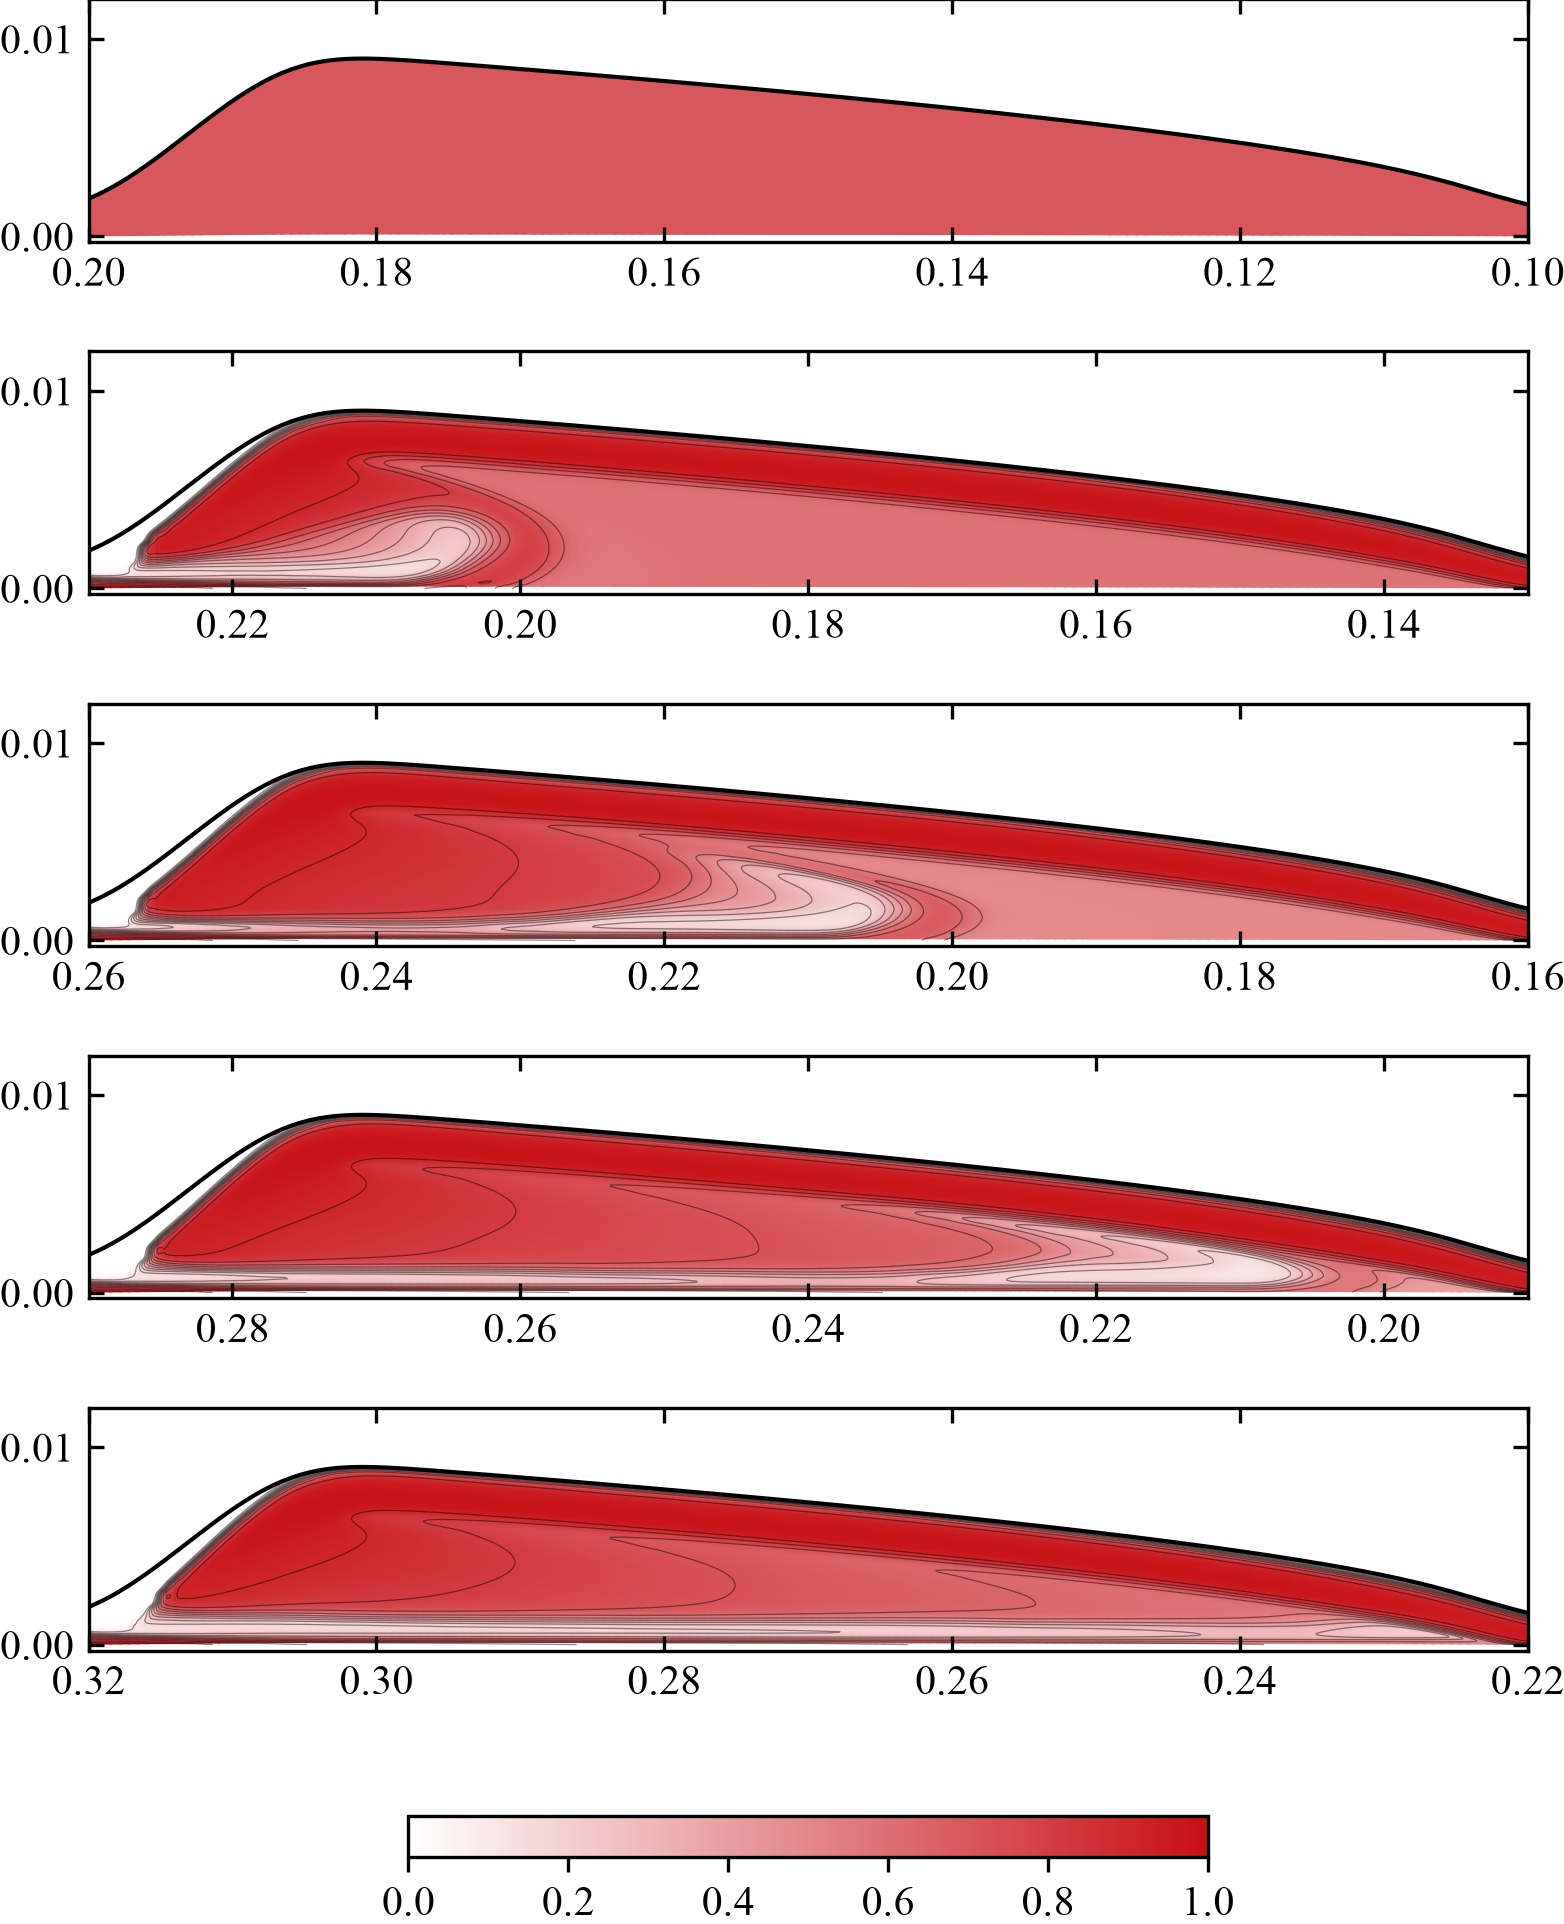
\includegraphics[width=0.8\linewidth]{figures/Slope_comparation_fan_i1_phi070.png}
    \caption{The evolving small-particle concentration $\phi_s$ at times (a) t = 0, (b) t = 600 s, (c) t = 1200 s, (d) t = 1800 s and (e) t = 2400 s. The black lines inside the dune show points where $\phi_s$ has the same value. The variables of this simulation are :$\phi_s = 70 \%$ and slope of the system of $i_1 = 0.97 \%$}
    \label{fig:fan_i1_phi070}
\end{figure}

%sounds weird
Figure \ref{fig:fan_i1_phi070} show the evolution of the fines concentration for $\phi_s^0 = 0.7$. Three features emerge in all of them, none of which is imposed by the initial condition~\eqref{eq:ic}, which is rigorously homogeneous and contains no pre-existing gradient or structure.

First, the mixture unmixes within the active layer and builds a coarse-rich
surface armour, which is then advected over the crest and deposited on the lee
face, restarting the cycle. Second, the deposit left behind is not uniform: it
retains a compositional stratification inherited from the avalanche cycle.
Third, a coarse-rich region becomes trapped beneath the active layer and,
when viewed in the frame that migrates with the bedform, remains essentially
stationary in $x$ until the dune front overtakes it.

%description of case phi_s = 0.90
%At the highest fines content (figure~\ref{fig:fan_i1_phi090}) the contour plots appear almost featureless. This is not a limitation of the visualization but a direct consequence of the closure: the segregation flux~\eqref{eq:Fseg} is proportional to $\phi_s(1-\phi_s)$ and therefore vanishes in both dilute limits, so a nearly monodisperse mixture has almost no segregation to perform. The few isoconcentration lines that do appear carry little information about the internal dynamics.

\subsection{Vertical sorting profiles}
\label{sec:res_sorting}

To move beyond this qualitative description we compress each run into a single
vertical profile by averaging $\phi_s$ along $x$ over the dune body, weighting
each column by its local thickness $h(x)$ so that the result is a volume
average rather than a column average,
\begin{equation}
\langle\phi_s\rangle_x(\eta)
  \;=\; \frac{\sum_x \phi_s(x,\eta)\,h(x)}{\sum_x h(x)} .
\label{eq:xaverage}
\end{equation}
%This is precisely the quantity measured in the flume experiments of \citet{blom2003} and parameterized in the sorting-evolution model of \citet{blom2008}, which makes it the natural point of contact between the present model and that body of work.

\begin{figure}
  \centering
  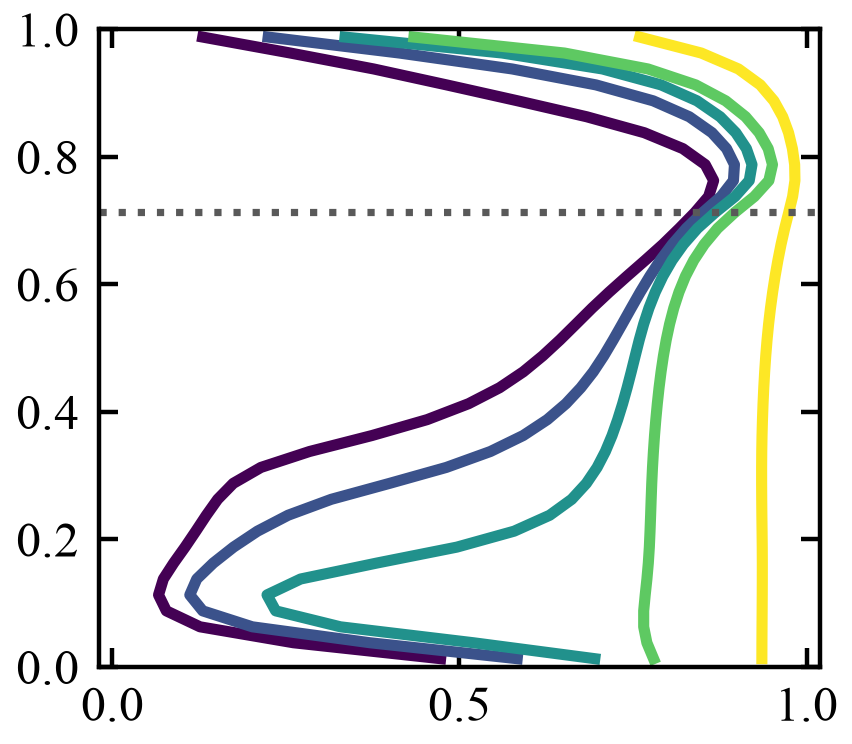
\includegraphics[width=0.4\linewidth]{figures/F1_a.png}
  \hfill
  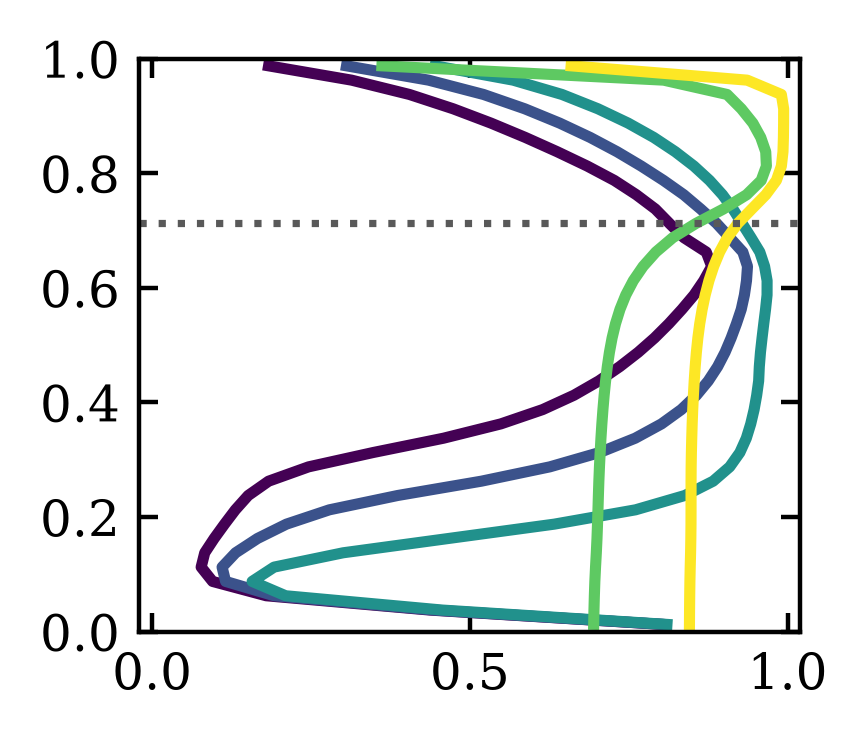
\includegraphics[width=0.4\linewidth]{figures/F1_b.png}
  \caption{Vertical sorting profiles $\langle\phi_s\rangle_x(\eta)$,
  eq.~\eqref{eq:xaverage}, at $t = 2400$~s for the five initial compositions.
  (\textit{a}) Full model with diffusion; dashed curves are the corresponding
  diffusive equilibrium profiles of \citet{graychugunov2006} evaluated within
  the active layer with $\ell = 0.135$~mm. (\textit{b}) Purely hyperbolic limit,
  eq.~\eqref{eq:hyperbolic}. The dotted horizontal line in (\textit{a},\textit{b}) marks the
  dune-averaged top of the buried deposit, $\langle\eta_a\rangle \simeq 0.71$.}
  \label{fig:sorting_profiles}
\end{figure}

Figure~\ref{fig:sorting_profiles}(\textit{a},\textit{b}) shows that every run
develops the same three-layer architecture: a coarse-rich base, a fines-rich
body, and a thin coarse crust at the free surface, visible as the reversal of
all curves when $\eta \approx 1$. The crust is the armour of
\S\ref{sec:res_architecture} caught in the act of being transported; the basal
coarse layer is what the lee-side grain flows have already buried. Superimposed
on panel~(\textit{a}) are the diffusive equilibrium profiles of
\citet{graychugunov2006} for the same mean composition. The simulated profiles
approach them near the free surface but depart from them below
$\langle\eta_a\rangle$, which confirms that the buried deposit is not a
relaxed equilibrium state: it is a record of the surface layer, frozen at the
moment of burial rather than allowed to equilibrate in place.

The grading index of figure~\ref{fig:sorting_profiles}(\textit{c}) turns this
into a single number per run,
\begin{equation}
\mathcal{G} \;=\;
  \langle\phi_s\rangle_{\mathrm{upper}} - \langle\phi_s\rangle_{\mathrm{lower}},
\label{eq:grading}
\end{equation}
each average being taken over one half of the buried deposit $\eta < \eta_a$.
Positive $\mathcal{G}$ means the deposit fines upward. The measured values are

\begin{center}
\footnotesize
\begin{tabular}{lccccc}
\toprule
$\phi_s^0$ & $0.5$ & $0.6$ & $0.7$ & $0.8$ & $0.9$ \\
\midrule
with diffusion & $+0.48$ & $+0.44$ & $+0.27$ & $+0.04$ & $+0.01$ \\
without diffusion & $+0.53$ & $+0.51$ & $+0.35$ & $+0.05$ & $+0.02$ \\
\bottomrule
\end{tabular}
\end{center}

\noindent
Two trends stand out. The index collapses monotonically towards zero as the
mixture becomes fines-dominated, quantifying the $\phi_s(1-\phi_s)$ argument of
\S\ref{sec:res_architecture}: a bidisperse bed can be structurally mute if its
composition is sufficiently far from equal proportions. And diffusion reduces
the grading by a systematic $\sim 20\%$ without altering the trend, consistent
with the role anticipated in \S\ref{sec:nodiff}, where $D_{sl}$ was argued to
control the internal degree of mixing of the laminae rather than their
position.

%%%%%%%%%%%%%% still for fix it
A terminological caution is in order. Equation~\eqref{eq:grading} measures {composition}, not sorting in the sedimentological sense of the arithmetic standard deviation ($\sigma_a$) used to quantify the spread of the mixture: for a bidisperse mixture, the arithmetic mean diameter $\bar{d} = (1-\phi_s)d_l + \phi_s d_s$ is monotonic in $\phi_s$, whereas the standard deviation of the grain size, $\sigma_d = \sqrt{\phi_s(1-\phi_s)}\,(d_l-d_s)$, is not, peaking at a fully mixed state of $\phi_s = 0.5$. A further caveat is that $\mathcal{G}$ carries a geometric bias: in the segregation-dominated limit, the sharp coarse--fine interface settles by mass balance at a height $\eta \simeq h\bar{\phi}_s$, so the contrast between halves is largest when that interface falls at mid-depth. The index is therefore a reliable indicator of the \emph{presence} of grading but not a discriminator of the segregation-velocity asymmetry contained in $F(R,\phi_s) = (R-1) + E(1-\phi_s)(R-1)^2$.

\subsection{The trapped coarse zone}
\label{sec:res_trapped}

The stationary coarse-rich region noted in \S\ref{sec:res_architecture} is the least intuitive feature of the simulations. 
%and deserves a mechanistic explanation. A natural first hypothesis is kinematic.
In the frame migrating with the dune, the horizontal velocity~\eqref{eq:u_horizontal} contains the constant $-c_{\mathrm{mig}}$, so the locus $u = 0$ separates material that
outruns the bedform from material that lags behind it and is buried. If the
trapped zone were simply the set of grains travelling at the dune celerity, it should coincide with that locus.

\begin{figure}
  \centerline{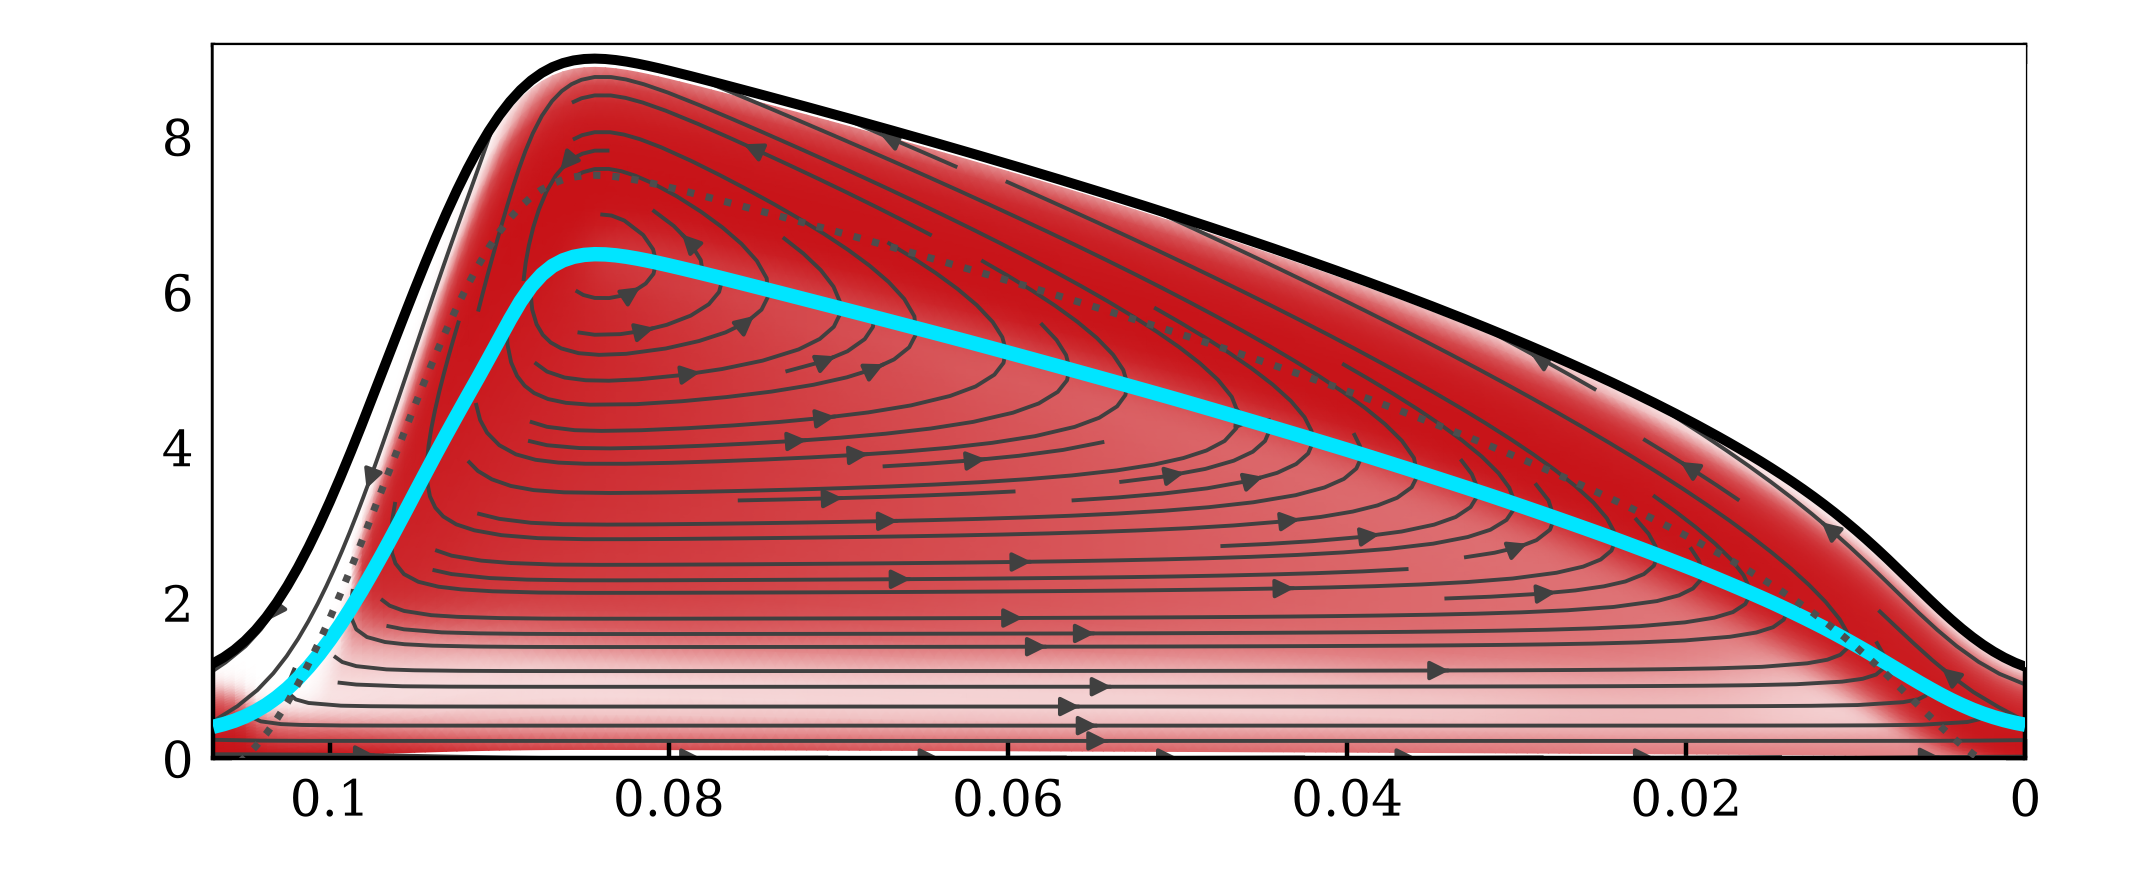
\includegraphics[width=1\textwidth]{figures/F2_a.png}}
  \vspace{6pt}
  \centerline{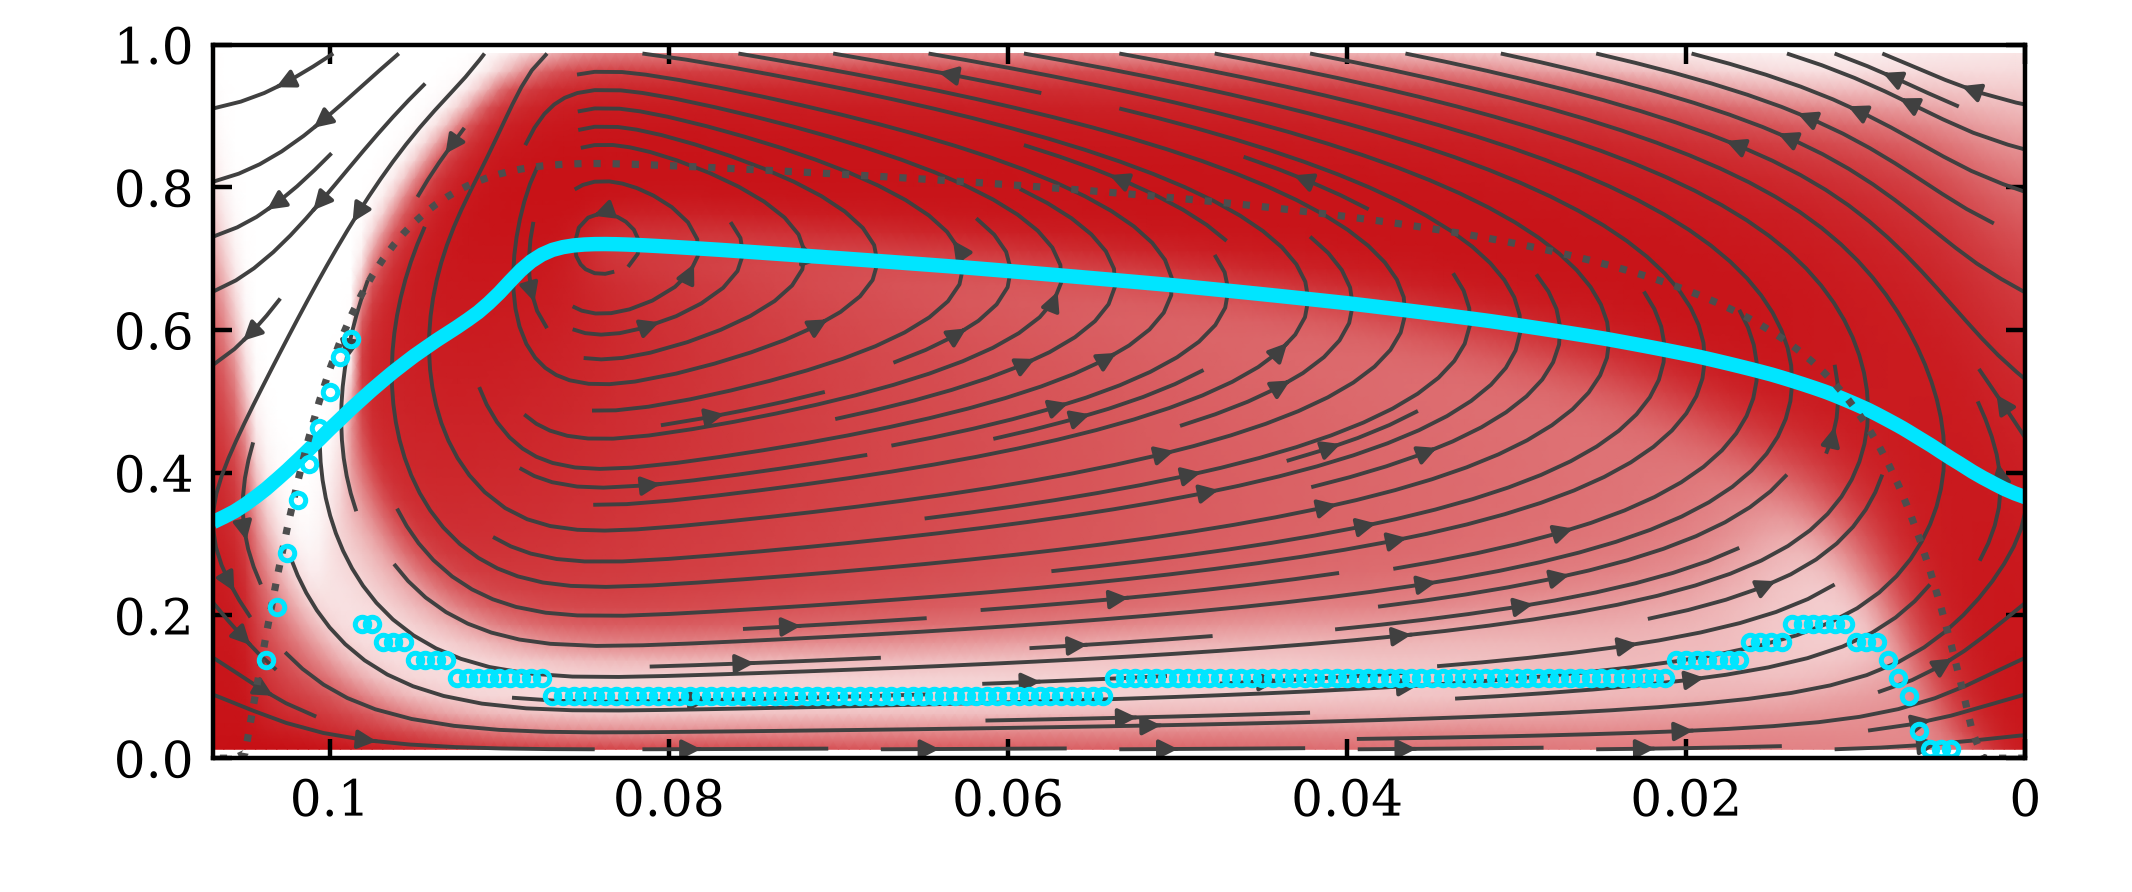
\includegraphics[width=1\textwidth]{figures/F2_b.png}}
  \caption{Fines concentration, streamlines of the dune-frame velocity field
  and the $u = 0$ contour (cyan) for $\phi_s^0 = 0.70$ at $t = 2400$~s, in
  (\textit{a}) physical coordinates $(x,z)$ and (\textit{b}) the
  computational $\sigma$-grid $(x,\eta)$. In (\textit{b}), open circles track
  the minimum of $\phi_s$ below $\eta_a$, i.e.\ the actual position of the
  trapped coarse zone, and the star marks the single genuine stagnation point
  where $u = 0$ and $w_\eta = 0$ simultaneously. The dotted line is the base of
  the active layer.}
  \label{fig:trapped_coarse}
\end{figure}
% more weirdo change it
Figure~\ref{fig:trapped_coarse} shows that the coarse
zone is located by the minimum of $\phi_s$ beneath $\eta_a$, rather than by a crossing of some fixed contour, because the isoline $\phi_s = 0.5$ possesses two branches (the surface armour and the basal layer) and is therefore not a unique locator. Measured over the $159$ columns of the dune body, the trapped zone lies a median of $0.53$ in $\eta$ \emph{below} the $u = 0$ contour, equivalent to $3.3$~mm, with a range of $[-0.10, +0.63]$; the two are moreover anticorrelated, with a Pearson coefficient of $-0.54$. Where $u = 0$ rises, the coarse material sits lower. The kinematic explanation is thus excluded.

The streamlines of panel~(\textit{b}) reveal the actual mechanism: the
dune-frame velocity field $(u, w_\eta)$ organizes into a \emph{closed
recirculation cell} centred near $x \approx 180$~mm, $\eta \approx 0.55$, with a single stagnation point at its core. Material advected into that cell cannot leave it by advection alone, and coarse grains that segregate upward into the cell are recirculated rather than expelled. The correct analogy in the granular literature is therefore not a kinematic stagnation point but the particle recirculation that accompanies breaking size-segregation waves \citep{Thornton2008}, and the time-dependent shock structures of \citet{gray2006time}. That such a structure arises here from a prescribed kinematic field, rather than from a fully coupled rheology
\citep{barker2021}, suggests it is a robust consequence of the closed
streamline topology of migrating bedforms and not a peculiarity of the
constitutive law.

\subsection{Why the structure freezes with depth}
\label{sec:res_freezing}

The equilibrium length $\ell$ of eq.~\eqref{eq:ell} was quoted in
\S\ref{sec:nodiff} as a single number for the reference configuration. It is
not, however, a constant: through the pressure $p(x,\eta)$ of
eq.~\eqref{eq:pressure} and the local composition it varies systematically
within the dune, and mapping that variation clarifies where in the deposit
segregation can still act.

\begin{figure}
  \centering
  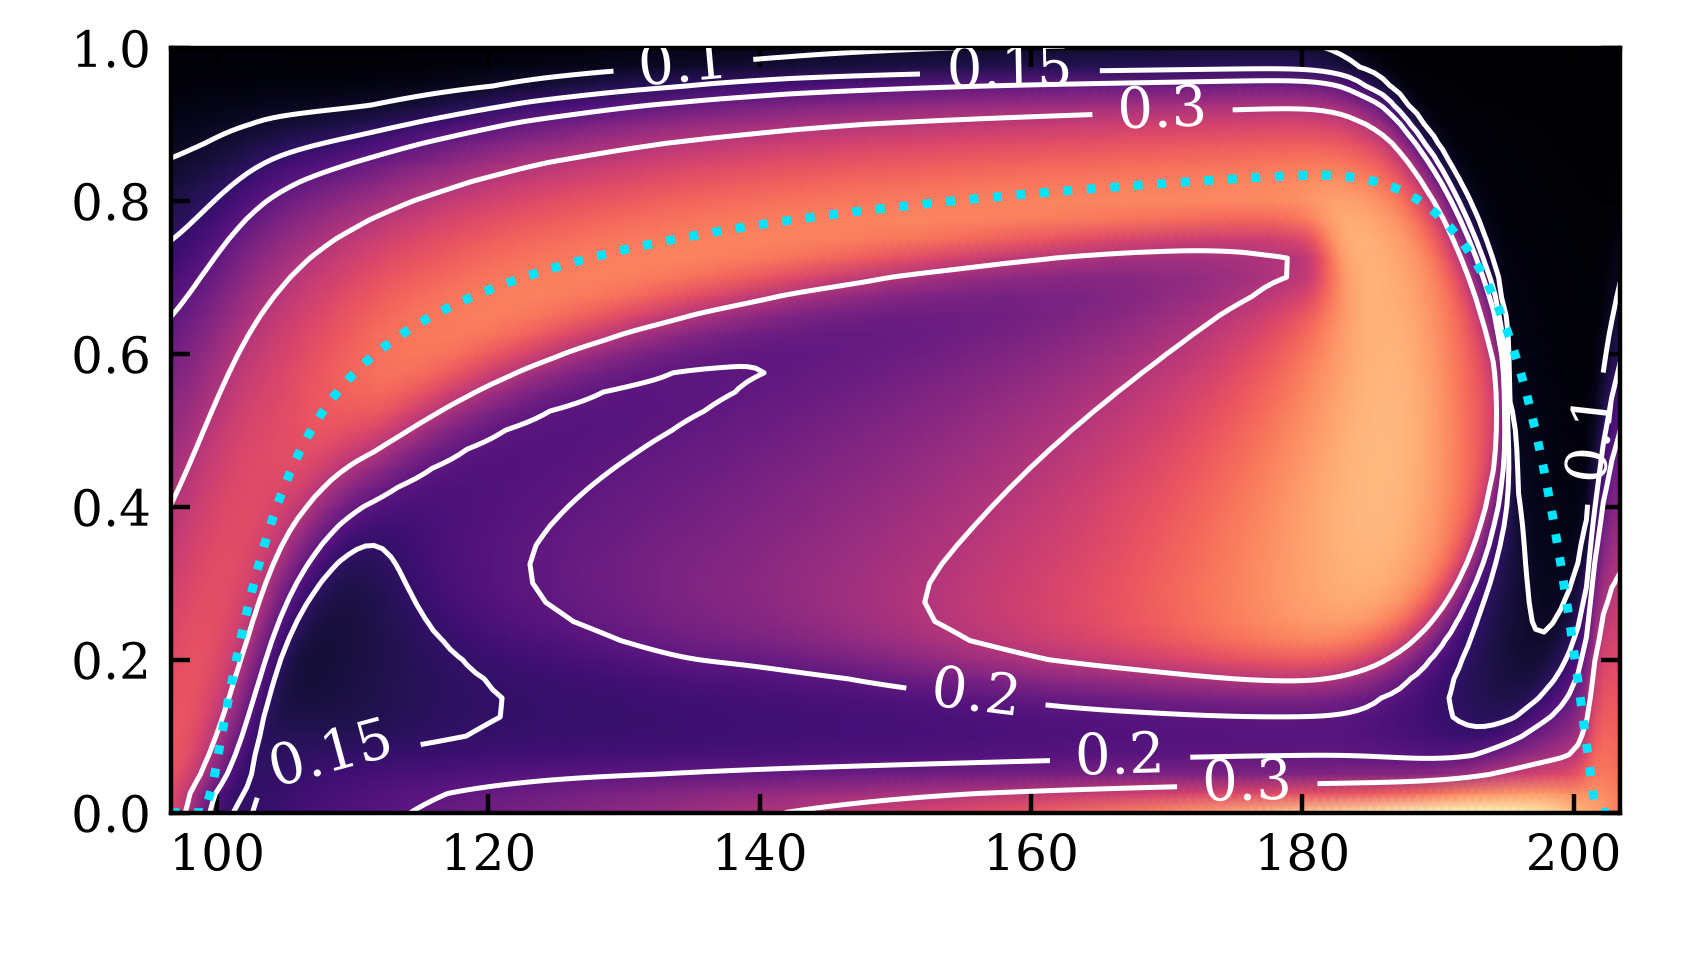
\includegraphics[width=0.49\linewidth]{figures/F4_a.png}
  \hfill
  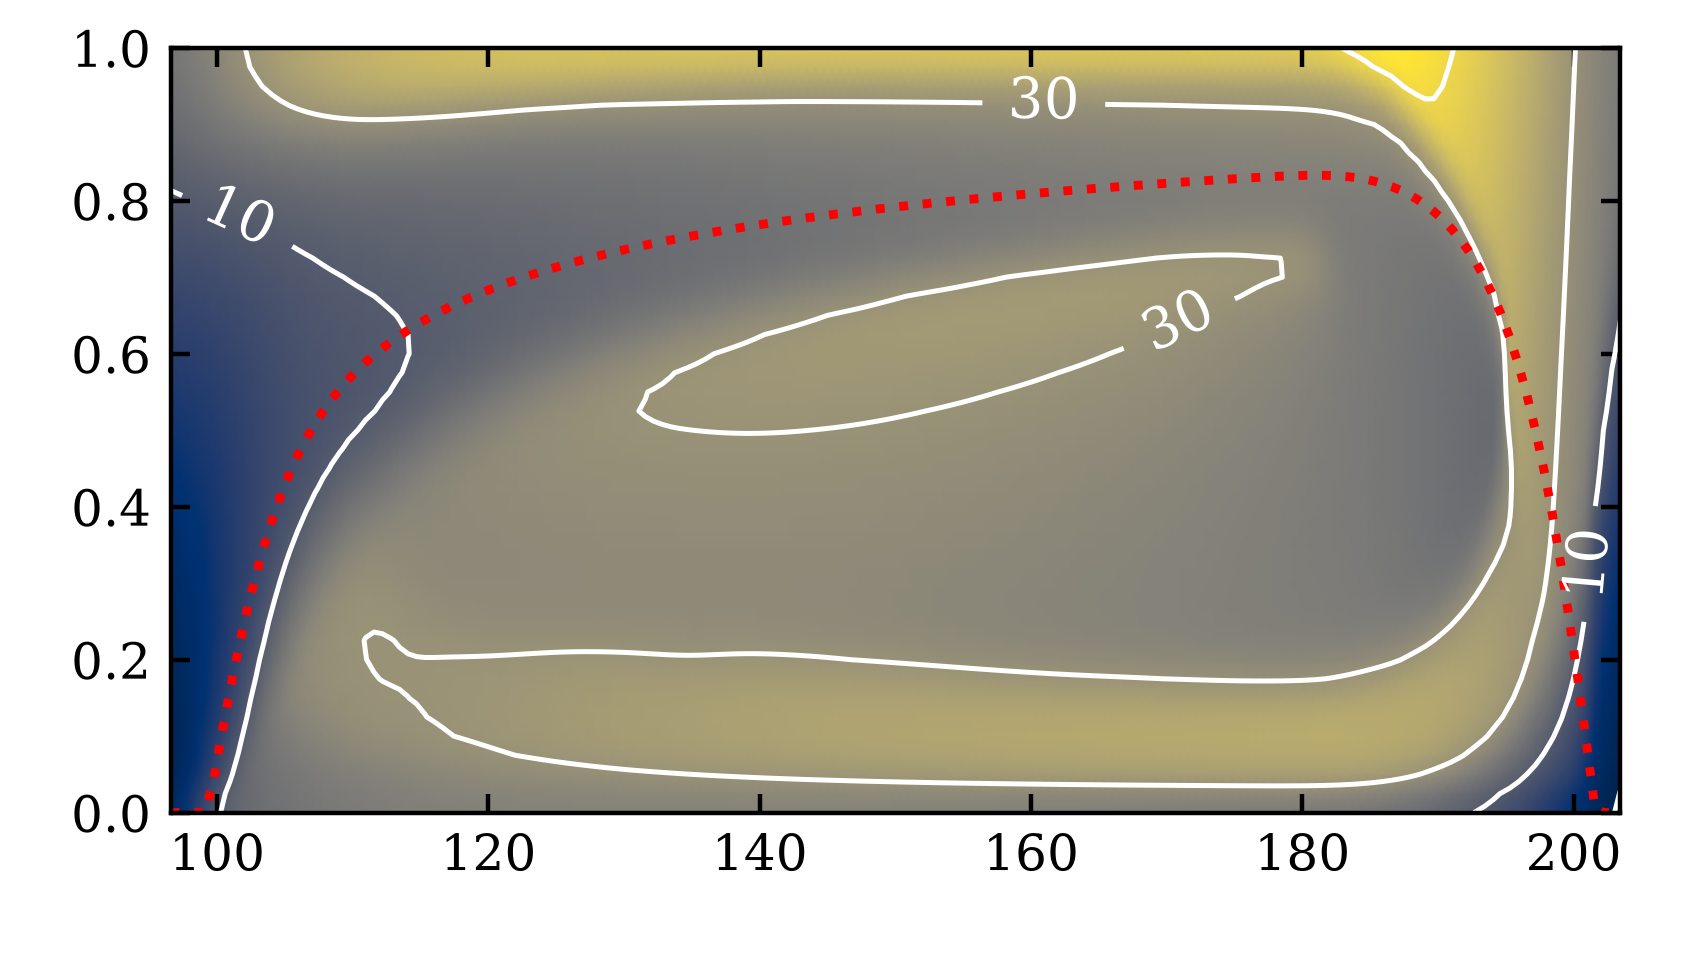
\includegraphics[width=0.49\linewidth]{figures/F4_b.png}
  \\[6pt]
  \caption{Segregation--diffusion balance within the dune for
  $\phi_s^0 = 0.70$ at $t = 2400$~s. (\textit{a}) Equilibrium length
  $\ell(x,\eta)$ of eq.~\eqref{eq:ell}, in mm. (\textit{b}) Local P\'eclet
  number $\mathrm{Pe} = h/\ell$.}
  \label{fig:ell_peclet}
\end{figure}

Because $\dot\gamma$ cancels between $f_{sl}$ and $D_{sl}$, neither $\ell$ nor $\mathrm{Pe}$ depends on the hydraulic slope; they are functions of composition and lithostatic pressure alone. Figure~\ref{fig:ell_peclet}(\textit{a},\textit{b}) shows the resulting structure: $\ell$ grows with depth as the overburden increases, and correspondingly $\mathrm{Pe}$ decreases downward and increases towards the crest, where $h$ is largest. At the reference column ($h = 4.98$~mm), $\ell/h$ rises from $0.013$ at the free surface to $0.109$ at the base, a factor of $8.7$; equivalently, $\mathrm{Pe} = h/\ell$ falls from $80$ to $9$, or from $24$ to $2.8$ when the active-layer thickness is used as the reference length instead.

This is a physically significant result for the interpretation of the model. The window $W_{\mathrm{act}}$ of eq.~\eqref{eq:Wact} was introduced as a modelling device to confine shear, and therefore segregation, to a surface layer; one could reasonably object that the observed freezing of the stratification is simply a consequence of that imposed window. Panels
(\textit{a},\textit{b}) show that it is not: the lithostatic pressure alone
already suppresses segregation at depth, so the structure would be preserved (more slowly, but preserved) even without $W_{\mathrm{act}}$. The prescribed window sharpens a transition that the physics of the closure produces on its own.

%Figure~\ref{fig:ell_peclet}(\textit{c}) also makes explicit a choice that is often left implicit. The P\'eclet number requires a reference length, and the two natural candidates answer different questions: $L = h$ asks whether segregation can organize the composition across the whole local flow depth, whereas $L = \delta_a$ restricts the question to the layer that is actually shearing, and is the relevant scale for deciding whether a lamina unmixes before it is buried. The offset between the two families of curves is $\delta_a/h$ and therefore varies along the bedform, from $0.18$ at the crest to $0.83$ at the lee toe, where the active layer occupies most of the column and the distinction all but disappears. Under either choice the system remains on the segregation-dominated side of $\mathrm{Pe} = 1$ throughout the column, although the margin narrows considerably towards the base.

%Panel~(\textit{d}) reports an honest limitation of the present parameterization. The pressure floor $p_{\mathrm{floor}} = 2.70\times10^{-3}$ introduced in eq.~\eqref{eq:pressure} to regularize the near-surface limit is of the same order as the maximum lithostatic pressure within the dune, $p_{\mathrm{lit}}^{\max} = 2.99\times10^{-3}$. Part of the depth dependence of $\ell$ is therefore regularization rather than physics, and the two curves of panel~(\textit{d}) bracket exactly how much. The qualitative conclusion --- that $\ell$ grows and $\mathrm{Pe}$ falls with depth --- survives the removal of thefloor, but the numerical factor of $8.7$ does not, and a thicker dune would be required to separate the two contributions cleanly.

\subsection{Approach to a travelling-wave state}
\label{sec:res_steady}

%comparing between t = 2400 s and t = 4800 s
\begin{figure}
  \centerline{\includegraphics[width=1\textwidth]{figures/t2400s_i1_phi070.png}}
  \vspace{6pt}
  \centerline{\includegraphics[width=1\textwidth]{figures/t4800s_phi070.png}}
  \caption{Approximate steady-state numerical solutions for the small-particle concentration $\phi_s = 70 \%$ when (\textit{a}) t = 2400 s (\textit{b}) t = 4800 s.}
  \label{fig:comparation between times}
\end{figure}

%In the frame co-moving with the bedform the problem admits, in principle, a travelling-wave solution, and figure~\ref{fig:comparation between times} suggests that the
simulations approach one: doubling the integration time from $2400$~s to $4800$~s leaves the internal architecture visually unchanged, with the coarse-rich band settling into a near-horizontal layer that runs from the lee face to beneath the fines-rich zone at the foot of the stoss side. Visual similarity, however, is a weak criterion, and it is worth replacing it with a measurement.

\begin{figure}
  \centering
  \includegraphics[width=0.87\linewidth]{figures/F6_b.png}
  \caption{Convergence towards the travelling-wave state for
  $\phi_s^0 = 0.70$. Collapse of the $x$-averaged sorting profile at nine instants
  between $0$ and $4800$~s; the dotted vertical line is the homogeneous initial
  condition of eq.~\eqref{eq:ic}.}
  \label{fig:convergence}
\end{figure}
%Eliminate F6a to pass a simple data or table isn't worth it make a figure about it


Figure~\ref{fig:convergence} shows the corresponding
behaviour of the $x$-averaged profile: the three latest curves, from $3000$ to
$4800$~s, are nearly superposed, whereas those between $600$ and $1800$~s remain
clearly distinct. The system slows markedly, and the surviving evolution is
confined to the interior of the deposit ratßher than to the active layer.

This evidence should not be over-interpreted, and the choice of normalization
matters. The denominator in panel~(\textit{a}) is the norm of the full field,
which for a quantity bounded in $[0,1]$ with a mean of $\langle\phi_s\rangle
\approx 0.67$ is dominated by that mean rather than by the structure. Referred
instead to the total change accumulated since the homogeneous initial
condition, the same difference between $t = 2400$~s and $t = 4800$~s amounts to
$11.5\%$. The deposit is therefore close to, but demonstrably not at, a
travelling-wave state on the timescale simulated here. Establishing statistical
steadiness would require covering many more avalanche cycles, and the residual
drift concerns the buried interior --- exactly the part of the solution that the
low-$\mathrm{Pe}$ region of figure~\ref{fig:ell_peclet} predicts should relax
most slowly.

\subsection{The diffusion-free limit}
\label{sec:res_nodiff}



Finally, figure~\ref{fig:diffusion_comparison} contrasts the full model with the singular limit $D_{sl} = 0$ of eq.~\eqref{eq:hyperbolic}, in which the smooth interfaces are replaced by genuine compositional shocks. The comparison confirms the role anticipated in \S\ref{sec:nodiff}: the two solutions place the coarse--fine interfaces at the same locations, but the hyperbolic run sustains a sharper contrast across them. The diffusion-free formulation therefore provides the upper bound on attainable compositional contrast, while the full model regularizes the same architecture towards the partially mixed laminations reported in flume experiments \citep{blom2003,kleinhans2004_34}.

This ordering is consistent with the regime diagnosed in
figure~\ref{fig:ell_peclet}: with $\mathrm{Pe} \gg 1$ throughout the column, granular diffusion is not competing with segregation for control of where the laminae form, only for how sharply they are expressed. One caveat must be attached to the comparison. At the working vertical resolution the physical interface thickness $\ell \approx 0.135$~mm is comparable to the grid spacing, so in the hyperbolic limit --- where no physical diffusion remains --- themeasured interface width is set partly by the numerical dissipation of theMUSCL--Rusanov scheme. The $20\%$ enhancement should therefore be read as alower bound on the true effect of $D_{sl}$.

\section{Conclusions}



\appendix

\section{Conservative formulation in the normalized vertical coordinate}
\label{app:conservative}

This appendix develops the transformation summarized at the end of \S\ref{sec:parameterization}: starting from the Cartesian form \eqref{eq:systemform} of the bidisperse segregation equation, we rewrite the differential operators in the normalized coordinate $\eta = z/h(x,t)$, introduce the coupled variable $h_\phi = h\,\phi_s$, and group the topographic gradients so that every vertical transport mechanism collapses under a single derivative in $\eta$. The result is the strictly conservative structural equation \eqref{eq:conservativa} that the numerical scheme of \S\ref{Sec:mathematical} integrates.

\subsection{Differential operators in normalized coordinates}
From the definition of the vertical variable $\eta = z/h(x,t)$, differentiating under the constraint of keeping the physical variable $z$ constant yields the following fundamental operator relations:
\begin{align}
    \frac{\partial \eta}{\partial z} &= \frac{1}{h}
    &&\Longrightarrow\quad
    {\frac{\partial}{\partial z} = \frac{1}{h}\frac{\partial}{\partial \eta}}, \label{eq:dz}\\[6pt]
    \frac{\partial \eta}{\partial x}\bigg|_z &= -\frac{z}{h^2}\frac{\partial h}{\partial x} = -\frac{\eta}{h}\frac{\partial h}{\partial x}
    &&\Longrightarrow\quad
    {\frac{\partial}{\partial x}\bigg|_z = \frac{\partial}{\partial x}\bigg|_\eta - \frac{\eta}{h}\frac{\partial h}{\partial x}\,\frac{\partial}{\partial \eta}}, \label{eq:dx}\\[6pt]
    \frac{\partial \eta}{\partial t}\bigg|_z &= -\frac{\eta}{h}\frac{\partial h}{\partial t}
    &&\Longrightarrow\quad
    {\frac{\partial}{\partial t}\bigg|_z = \frac{\partial}{\partial t}\bigg|_\eta - \frac{\eta}{h}\frac{\partial h}{\partial t}\,\frac{\partial}{\partial \eta}}. \label{eq:dt}
\end{align}

\subsection{Substitution of operators in the Cartesian equation}
Substituting the operators defined in \eqref{eq:dz}--\eqref{eq:dt} into each term of the Cartesian differential equation \eqref{eq:systemform} yields:
\begin{align}
    \frac{\partial \phi_s}{\partial t} &= \frac{\partial \phi_s}{\partial t} - \frac{\eta}{h}\frac{\partial h}{\partial t}\frac{\partial \phi_s}{\partial \eta}, \\
    \frac{\partial (u\phi_s)}{\partial x} &= \frac{\partial (u\phi_s)}{\partial x} - \frac{\eta}{h}\frac{\partial h}{\partial x}\frac{\partial (u\phi_s)}{\partial \eta}, \\
    \frac{\partial (w\phi_s)}{\partial z} &= \frac{1}{h}\frac{\partial (w\phi_s)}{\partial \eta}, \qquad
    \frac{\partial F_{\mathrm{seg}}}{\partial z} = \frac{1}{h}\frac{\partial F_{\mathrm{seg}}}{\partial \eta}, \\
    \frac{\partial}{\partial z}\!\left(D_{\mathrm{sl}}\frac{\partial \phi_s}{\partial z}\right) &= \frac{1}{h}\frac{\partial}{\partial \eta}\!\left(\frac{D_{\mathrm{sl}}}{h}\frac{\partial \phi_s}{\partial \eta}\right).
\end{align}
Grouping the terms above, setting the resulting expression equal to zero, and multiplying by the scalar factor $h$ eliminates the fractional dependence on thickness:
\begin{multline}
    h\frac{\partial \phi_s}{\partial t} - \eta\,\frac{\partial h}{\partial t}\frac{\partial \phi_s}{\partial \eta}
    + h\frac{\partial (u\phi_s)}{\partial x} - \eta\,\frac{\partial h}{\partial x}\frac{\partial (u\phi_s)}{\partial \eta} \\
    + \frac{\partial (w\phi_s)}{\partial \eta} + \frac{\partial F_{\mathrm{seg}}}{\partial z}h - \frac{\partial}{\partial \eta}\!\left(\frac{D_{\mathrm{sl}}}{h}\frac{\partial \phi_s}{\partial \eta}\right) = 0.
    \label{eq:ast}
\end{multline}

\subsection{Introduction of the coupled variable $h_{\phi}$}
Since the topographic variable $h$ is independent of the normalized vertical position $\eta$, applying the product rule in reverse yields the following differential identities:
\begin{align}
    \frac{\partial h_{\phi}}{\partial t} = \frac{\partial (h\phi_s)}{\partial t} = h\frac{\partial \phi_s}{\partial t} + \phi_s\frac{\partial h}{\partial t}
    &\;\Longrightarrow\; h\frac{\partial \phi_s}{\partial t} = \frac{\partial h_{\phi}}{\partial t} - \phi_s\frac{\partial h}{\partial t}, \label{eq:idQt}\\
    \frac{\partial (u\,h_{\phi})}{\partial x} = \frac{\partial (hu\phi_s)}{\partial x} = h\frac{\partial (u\phi_s)}{\partial x} + u\phi_s\frac{\partial h}{\partial x}
    &\;\Longrightarrow\; h\frac{\partial (u\phi_s)}{\partial x} = \frac{\partial (u\,h_{\phi})}{\partial x} - u\phi_s\frac{\partial h}{\partial x}. \label{eq:idQx}
\end{align}
Substituting equations \eqref{eq:idQt} and \eqref{eq:idQx} into the expanded expression \eqref{eq:ast} gives
\begin{multline}
    \left[\frac{\partial h_{\phi}}{\partial t} - \phi_s\frac{\partial h}{\partial t}\right] - \eta\,\frac{\partial h}{\partial t}\frac{\partial \phi_s}{\partial \eta}
    + \left[\frac{\partial (u\,h_{\phi})}{\partial x} - u\phi_s\frac{\partial h}{\partial x}\right] - \eta\,\frac{\partial h}{\partial x}\frac{\partial (u\phi_s)}{\partial \eta} \\
    + \frac{\partial (w\phi_s)}{\partial \eta} + \frac{\partial F_{\mathrm{seg}}}{\partial \eta}
    - \frac{\partial}{\partial \eta}\!\left(\frac{D_{\mathrm{sl}}}{h}\frac{\partial \phi_s}{\partial \eta}\right) = 0.
    \label{eq:paso3}
\end{multline}

\subsection{Grouping of topographic gradients}
The terms containing time derivatives of topography are consolidated using the identity $\partial(\eta\phi_s)/\partial\eta = \phi_s + \eta\,\partial\phi_s/\partial\eta$:
\begin{equation}
    -\phi_s\frac{\partial h}{\partial t} - \eta\,\frac{\partial h}{\partial t}\frac{\partial \phi_s}{\partial \eta}
    = -\frac{\partial h}{\partial t}\left[\phi_s + \eta\frac{\partial \phi_s}{\partial \eta}\right]
    = -\frac{\partial}{\partial \eta}\!\left(\eta\,\phi_s\,\frac{\partial h}{\partial t}\right).
    \label{eq:grupo_t}
\end{equation}
Similarly, the spatial gradients of thickness combine as
\begin{equation}
    -u\phi_s\frac{\partial h}{\partial x} - \eta\,\frac{\partial h}{\partial x}\frac{\partial (u\phi_s)}{\partial \eta}
    = -\frac{\partial}{\partial \eta}\!\left(\eta\,u\,\phi_s\,\frac{\partial h}{\partial x}\right).
    \label{eq:grupo_x}
\end{equation}

\subsection{Consolidation under the vertical operator}
Introducing simplifications \eqref{eq:grupo_t} and \eqref{eq:grupo_x} into the base equation \eqref{eq:paso3} unifies the governing fluxes under a single gradient with respect to $\eta$:
\begin{equation}
    \frac{\partial h_{\phi}}{\partial t} + \frac{\partial (u\,h_{\phi})}{\partial x} + \frac{\partial}{\partial \eta}\left[\, w\phi_s - \eta\,\phi_s\frac{\partial h}{\partial t} - \eta\,u\,\phi_s\frac{\partial h}{\partial x} + F_{\mathrm{seg}} - \frac{D_{\mathrm{sl}}}{h}\frac{\partial \phi_s}{\partial \eta} \,\right] = 0.
    \label{eq:paso5}
\end{equation}
Factoring out the common concentration term $\phi_s$ shows that the advective component matches the flux definition given in \eqref{eq:Fadv}:
\begin{equation}
    w\phi_s - \eta\,\phi_s\frac{\partial h}{\partial t} - \eta\,u\,\phi_s\frac{\partial h}{\partial x} = \left(w - \eta\frac{\partial h}{\partial t} - \eta\,u\frac{\partial h}{\partial x}\right)\phi_s \equiv F_{\mathrm{adv},\eta}.
\end{equation}

Redefining the physical flux functions accordingly recovers the conservative structural equation \eqref{eq:conservativa} quoted in \S\ref{sec:parameterization}, with the constitutive fluxes \eqref{eq:Fadv}--\eqref{eq:Fdiff} defined there. The derivation is exact: no term has been neglected in passing from the Cartesian formulation \eqref{eq:systemform} to the transformed one, so the conservation of the mass of fines guaranteed by the variable $h_\phi$ is inherited in full by the transformed equation, and with it by the discrete scheme built upon it.

\section{Weighted Essentially Non-Oscillatory 5}
\label{app:weno5}

This appendix develops the horizontal spatial discretization summarized in \S\ref{sec:weno5}: the upwind principle that underlies the advective fluxes of the model, the fifth-order WENO reconstruction used to supply the interface states, and the way both combine into the conserved flux and the spatial operator $R_x$ that the SSP Runge--Kutta scheme integrates in time.

%UPWIND
The upwind principle underlies the advective discretization throughout the model, both horizontally and vertically. Inherited from Godunov's method \citep{Godunov1959}, its logic respects the physical direction of information propagation: the numerical flux at an interface is built from the upstream state -- the side from which the velocity transports the concentration. In its simplest form, for an advection velocity $a$, the numerical flux at face $i+\tfrac{1}{2}$ is
\begin{equation}
    F_{i+1/2} =
    \begin{cases}
        a\,\phi_i & \text{if } a \geq 0 \ (\text{upstream: cell } i), \\
        a\,\phi_{i+1} & \text{if } a < 0 \ (\text{upstream: cell } i+1),
    \end{cases}
    \label{eq:upwind_basic}
\end{equation}
which can be written compactly by splitting the velocity into positive and negative parts, $a = a^+ + a^-$, with $a^+=\max(a,0)$ and $a^-=\min(a,0)$:
\begin{equation}
    F_{i+1/2} = a^+ \phi_i + a^- \phi_{i+1}.
    \label{eq:upwind_compact}
\end{equation}
This choice introduces implicit numerical dissipation that stabilizes the transport and prevents $\phi_s$ from leaving the physical range, unlike a centred scheme, which would be unstable for pure advection \citep{Godunov1959}. Taken on its own, however, the criterion \eqref{eq:upwind_compact} evaluates the flux from cell-centred values and is therefore only first-order accurate, and the numerical dissipation it introduces is of the order of the grid spacing. Applied to the horizontal transport of the model, over the thousands of time steps required to migrate a dune, such a scheme would smear the compositional laminae well before they could be compared with the experimental deposit. The sign-based selection is therefore retained, but the states feeding it are supplied by a high-order reconstruction rather than by the cell averages themselves.

%WENO
To describe the WENO5 finite-difference scheme, consider a uniform spatial discretization with nodes $x_i$ and grid spacing $\Delta x$. The goal is to approximate the flux derivative at each node from the numerical fluxes reconstructed at the interfaces $x_{i\pm1/2}$:
\begin{equation}
    \frac{\partial (u h_\phi)}{\partial x}\bigg|_{x_i} \approx \frac{\hat f_{i+1/2} - \hat f_{i-1/2}}{\Delta x},
    \label{eq:weno_deriv}
\end{equation}
where, for notational simplicity, we define $f \equiv u h_\phi$, so that $f_{i\pm1/2} = (u h_\phi)_{i\pm1/2}$. To reconstruct the numerical flux at the interface $\hat f_{i+1/2}$, the WENO5 scheme uses a global five-point stencil, $S_5 = \{x_{i-2},x_{i-1},x_i,x_{i+1},x_{i+2}\}$, split into three three-point sub-stencils ($r=3$):
\begin{equation}
    S_0 = \{x_{i-2},x_{i-1},x_i\}, \quad S_1 = \{x_{i-1},x_i,x_{i+1}\}, \quad S_2 = \{x_i,x_{i+1},x_{i+2}\}.
    \label{eq:substencils}
\end{equation}
Each sub-stencil generates a third-order polynomial approximation of the numerical flux, denoted $\hat f_{i+1/2}^{(k)}$ for $k=0,1,2$:
\begin{align}
    \hat f_{i+1/2}^{(0)} &= \tfrac{1}{3} f_{i-2} - \tfrac{7}{6} f_{i-1} + \tfrac{11}{6} f_i, \label{eq:f0}\\
    \hat f_{i+1/2}^{(1)} &= -\tfrac{1}{6} f_{i-1} + \tfrac{5}{6} f_i + \tfrac{1}{3} f_{i+1}, \label{eq:f1}\\
    \hat f_{i+1/2}^{(2)} &= \tfrac{1}{3} f_i + \tfrac{5}{6} f_{i+1} - \tfrac{1}{6} f_{i+2}. \label{eq:f2}
\end{align}
If the solution is smooth across the entire global stencil $S_5$, these three local reconstructions can be linearly combined using the ``optimal'' or linear weights $d_k$, yielding a fifth-order approximation that emulates a maximal-order upwind scheme \citep{JiangShu1996}:
\begin{equation}
    \hat f_{i+1/2} = d_0\, \hat f_{i+1/2}^{(0)} + d_1\, \hat f_{i+1/2}^{(1)} + d_2\, \hat f_{i+1/2}^{(2)},
    \label{eq:weno_combo}
\end{equation}
with $d_0 = 1/10$, $d_1 = 3/5$, and $d_2 = 3/10$. Near discontinuities, however, the linear weights must be replaced by nonlinear weights $\omega_k$ that adapt dynamically to the local smoothness of the solution. These weights follow from normalizing the intermediate weights $\alpha_k$:
\begin{equation}
    \omega_k = \frac{\alpha_k}{\sum_{l=0}^{2} \alpha_l}, \qquad
    \alpha_k = \frac{d_k}{(\beta_k + \epsilon)^p},
    \label{eq:nonlinear_weights}
\end{equation}
where $\epsilon = 10^{-6}$ regularizes against division by zero, $p=2$ is an integer exponent that sharpens the rejection of non-smooth sub-stencils, and $\beta_k$ is the smoothness indicator of sub-stencil $S_k$. \citet{JiangShu1996} defined these indicators from the sum of the $L^2$ norms of the derivatives of the reconstruction polynomial $q_k(x)$ over the integration cell:
\begin{equation}
    \beta_k = \sum_{l=1}^{r-1} \int_{x_{i-1/2}}^{x_{i+1/2}} \Delta x^{2l-1} \left(\frac{\mathrm{d}^l q_k(x)}{\mathrm{d}x^l}\right)^2 \mathrm{d}x.
    \label{eq:beta_general}
\end{equation}
Evaluating these integrals explicitly for $r=3$ yields the classical Jiang--Shu algebraic expressions for the smoothness indicators \citep{JiangShu1996}:
\begin{align}
    \beta_0 &= \tfrac{13}{12}(f_{i-2}-2f_{i-1}+f_i)^2 + \tfrac{1}{4}(f_{i-2}-4f_{i-1}+3f_i)^2, \label{eq:beta0}\\
    \beta_1 &= \tfrac{13}{12}(f_{i-1}-2f_i+f_{i+1})^2 + \tfrac{1}{4}(f_{i-1}-f_{i+1})^2, \label{eq:beta1}\\
    \beta_2 &= \tfrac{13}{12}(f_i-2f_{i+1}+f_{i+2})^2 + \tfrac{1}{4}(3f_i-4f_{i+1}+f_{i+2})^2. \label{eq:beta2}
\end{align}
A discontinuity within a local sub-stencil thus produces a large smoothness indicator ($\beta_k = O(1)$), which drives the associated nonlinear weight $\omega_k$ toward a negligible value and suppresses numerical oscillations near the shock. In smooth regions, the weights converge to the optimal values $d_k$ and the scheme recovers its nominal fifth order (with numerical dissipation of order $\sim\Delta x^5$) while at sharp fronts it locally degrades the reconstruction order in the affected sub-stencil to avoid the Gibbs phenomenon \citep{JiangShu1996}. The reconstructed flux is then obtained by replacing the linear weights of \eqref{eq:weno_combo} with their nonlinear counterparts,
\begin{equation}
    \hat f_{i+1/2} = \omega_0\, \hat f_{i+1/2}^{(0)} + \omega_1\, \hat f_{i+1/2}^{(1)} + \omega_2\, \hat f_{i+1/2}^{(2)},
    \label{eq:weno_nonlinear_combo}
\end{equation}
which by construction satisfies $\sum_k \omega_k = 1$ with $\omega_k \geq 0$. The combination is therefore convex, so the reconstruction remains consistent whatever the local smoothness and cannot generate values outside the range spanned by the three candidates. The stencils \eqref{eq:substencils} are biased toward the left, which is the correct choice when the transport velocity is positive; for a negative velocity the whole construction is mirrored about the interface, so that the five-point stencil becomes $\{x_{i+3},\dots,x_{i-1}\}$ and the candidate reconstructions read the solution from downstream to upstream in the same order. In the model, both branches are evaluated at every face, producing the two states $\phi^{L}$ and $\phi^{R}$, and the upwind criterion of \eqref{eq:upwind_compact} decides which one enters the flux. Because the domain is periodic in $x$ (\S\ref{sec:ic}), the five-point stencil is closed at the boundaries with three ghost cells on each side copied from the opposite end of the domain, so no reduction of the reconstruction order is needed near the edges of the grid.

Combining the two ingredients gives the conserved horizontal flux of the model. The advective velocity is averaged to the faces, $u_{i+1/2}=\tfrac{1}{2}(u_i+u_{i+1})$, the WENO5 states $\phi^{L}$ and $\phi^{R}$ are reconstructed on either side of the interface, and the upstream one is selected according to the sign of $u_{i+1/2}$:
\begin{equation}
    F_{i+1/2} =
    \begin{cases}
        u_{i+1/2}\, \phi^L\, h_i & \text{if } u_{i+1/2} \geq 0, \\
        u_{i+1/2}\, \phi^R\, h_{i+1} & \text{if } u_{i+1/2} < 0,
    \end{cases}
    \label{eq:horiz_flux}
\end{equation}
where $h$ is the local layer thickness, which enters because the transported variable is the conserved quantity $h_\phi$ rather than the concentration itself. The thickness is evaluated in the upstream cell as well, so that the flux leaving a cell is exactly the flux entering its neighbour and the discrete mass of fines is conserved to machine precision. The horizontal spatial operator follows as the discrete divergence of these fluxes,
\begin{equation}
    R_x = -\frac{F_{i+1/2}-F_{i-1/2}}{\Delta x},
    \label{eq:Rx}
\end{equation}
which is the term integrated in time by the two-stage SSP Runge--Kutta scheme \eqref{eq:rk_stage1}--\eqref{eq:rk_stage2}. The pairing is deliberate: the SSP property guarantees that the non-oscillatory character built into the nonlinear weights is not destroyed by the time advance, provided the horizontal step respects the CFL bound \eqref{eq:cflh}. Together, \eqref{eq:horiz_flux} and \eqref{eq:Rx} keep the compositional laminae sharp along the stoss flank, where the solution is smooth and the fifth-order accuracy is effective, while preventing spurious oscillations at the crest and the lee-side toe, where the concentration field develops the steep fronts discussed in \S\ref{sec:weno5}.

\newpage
\bibliographystyle{jfm}
\bibliography{jfm}

%Use of the above commands will create a bibliography using the .bib file. Shown below is a bibliography built from individual items.


%% End of file `jfm.bib'.


\end{document}